\documentclass{jsarticle}

\usepackage[dvipdfmx]{graphicx}

\title{ベニシジミ観察日誌}

\begin{document}
\maketitle

\section{5/11の記録}

\subsection{16時:採集}
自宅付近の, 北八朔町1627-12付近にある, 狭い公園にて, 16時前後. 
公園で, 食痕のあるスイバの葉を何枚か裏返すものの, 見つかるのは, 写真\ref{pic-hagurohabachi}の, ハグロハバチと思われる, 細長い幼虫ばかりであった. 
\begin{figure}[htbp]
  \begin{center}
    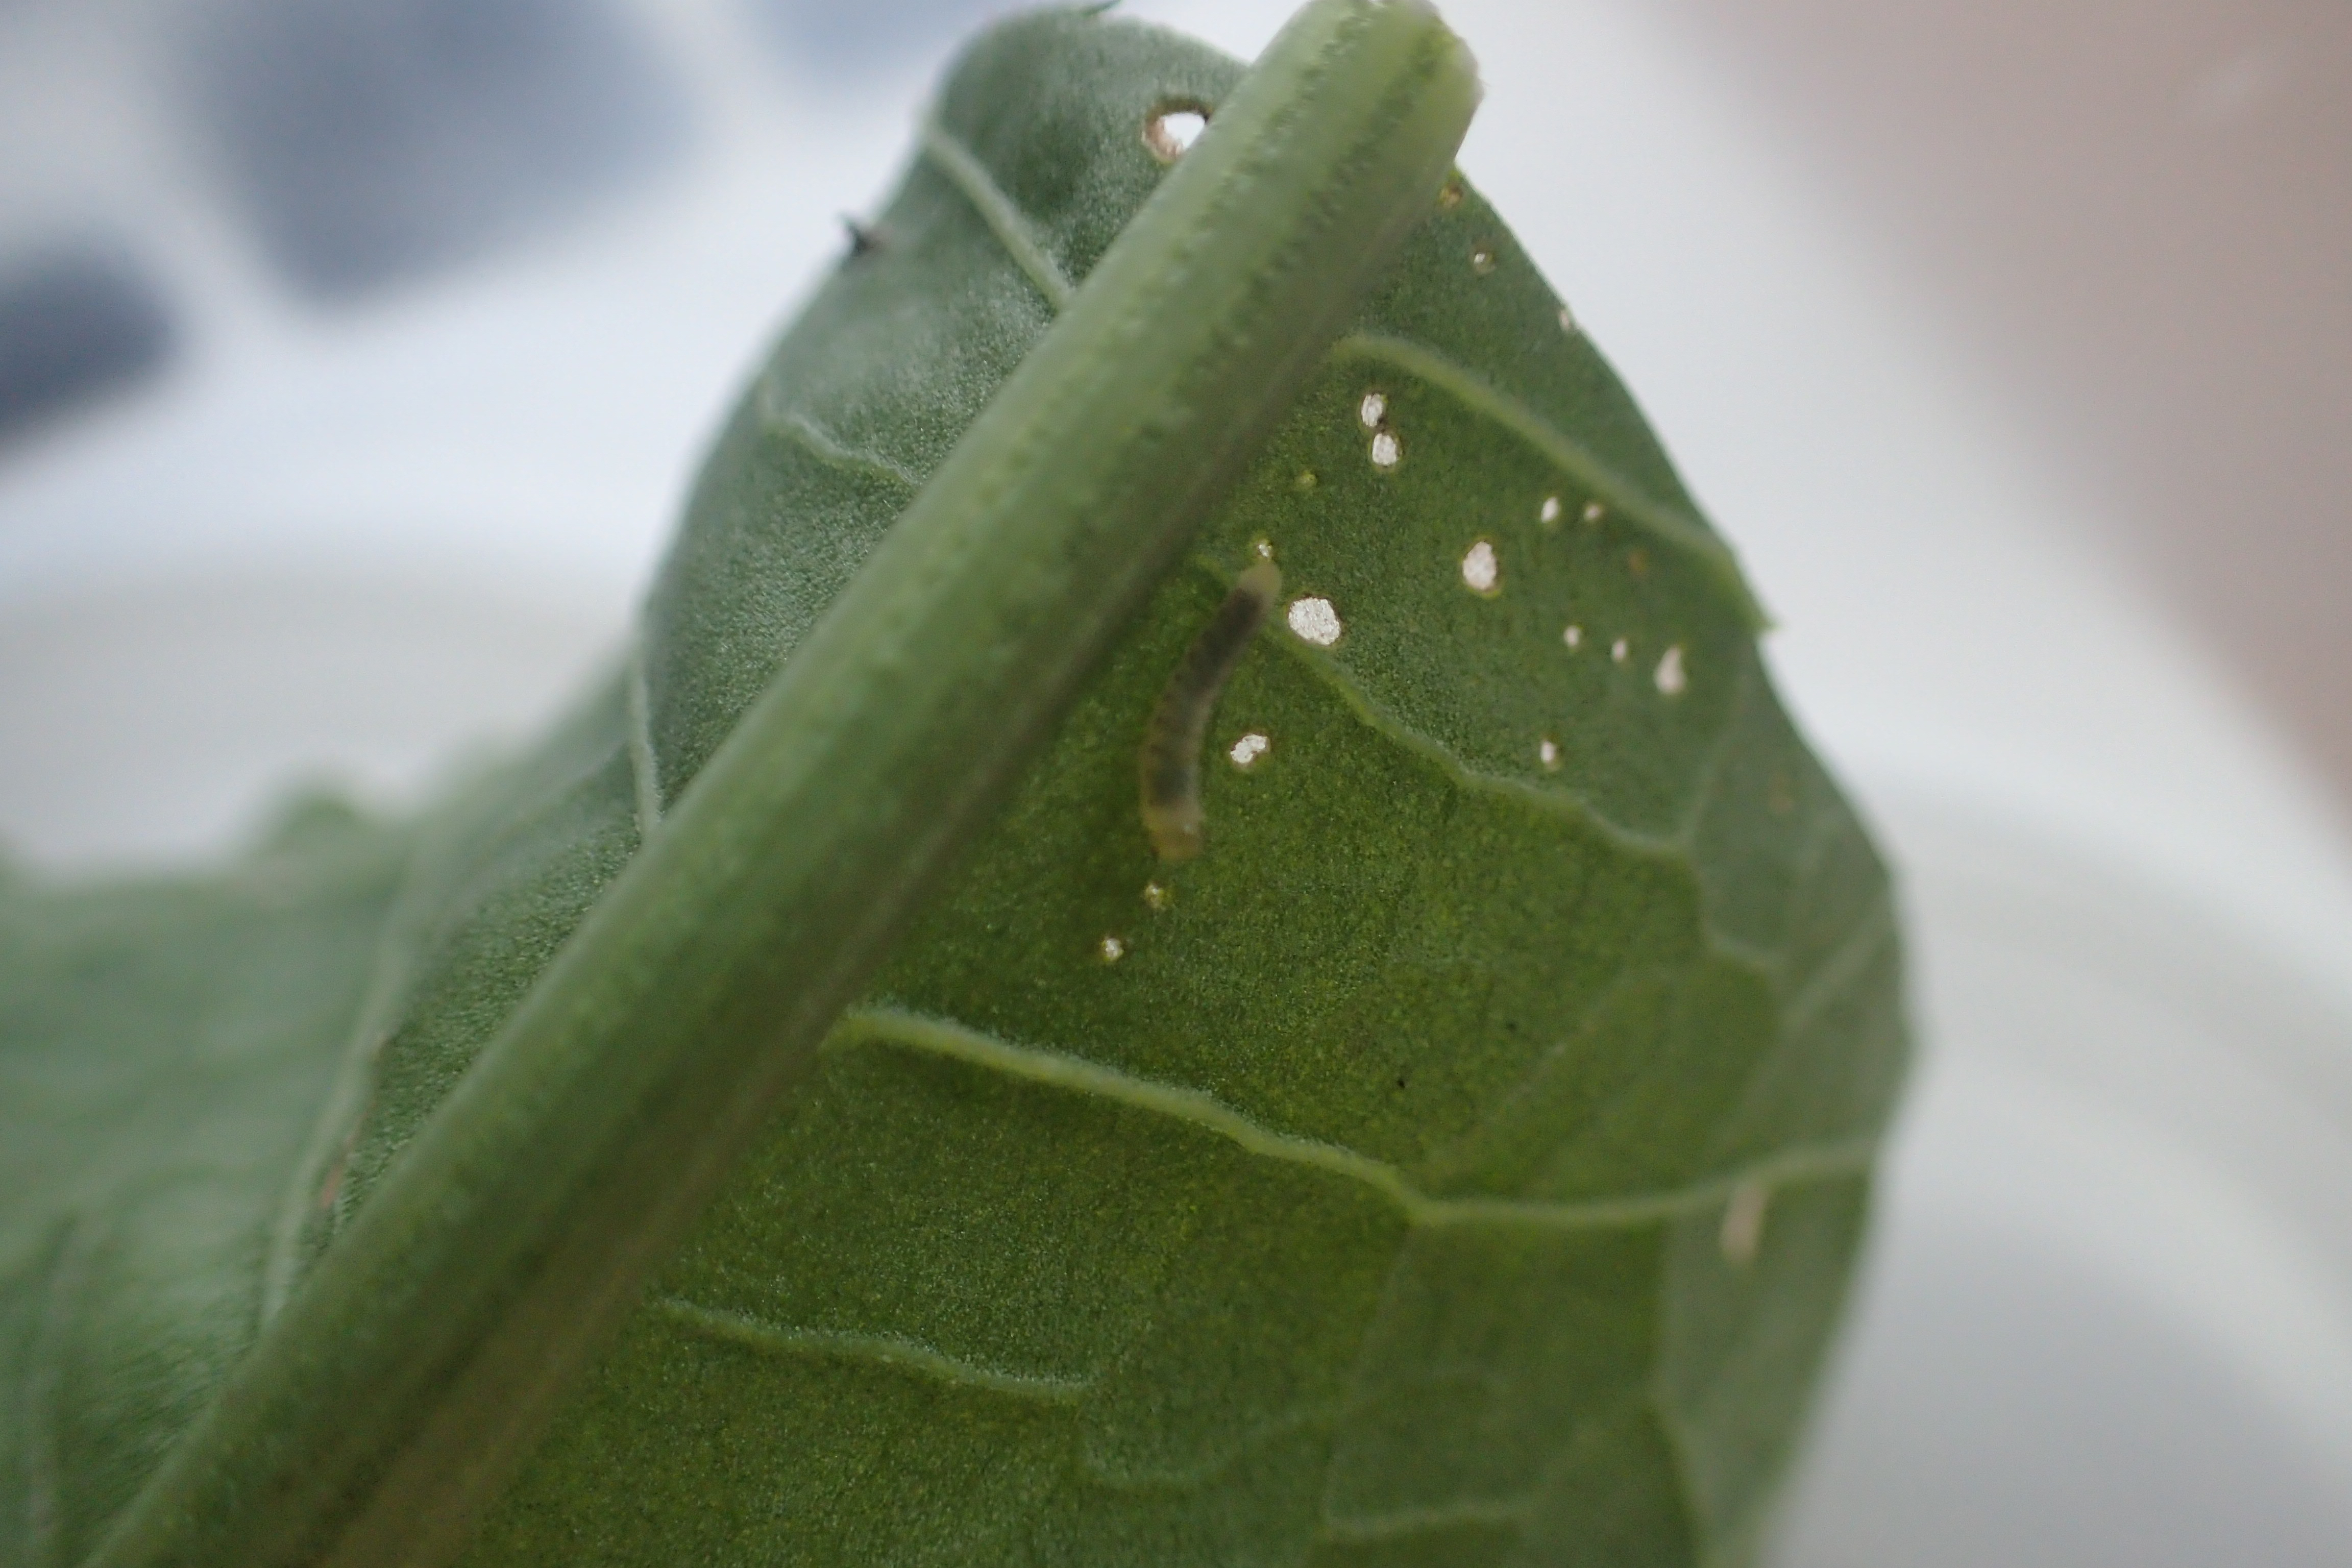
\includegraphics[width=5cm]{photo/hagurohabachi1.JPG}
    \caption{スイバの葉裏でよく見つかったハグロハバチと思われる幼虫}
    \label{pic-hagurohabachi}
  \end{center}
\end{figure}

そのまま, 公園の奥の方にスイバがまばらに生えている方に向かったところ, ほとんど葉がないスイバの, かなり上の方に, ぼてっとした幼虫が写真\ref{pic-sitting-on-branch}のように, とまっているのを発見. 
\begin{figure}[htbp]
  \begin{center}
    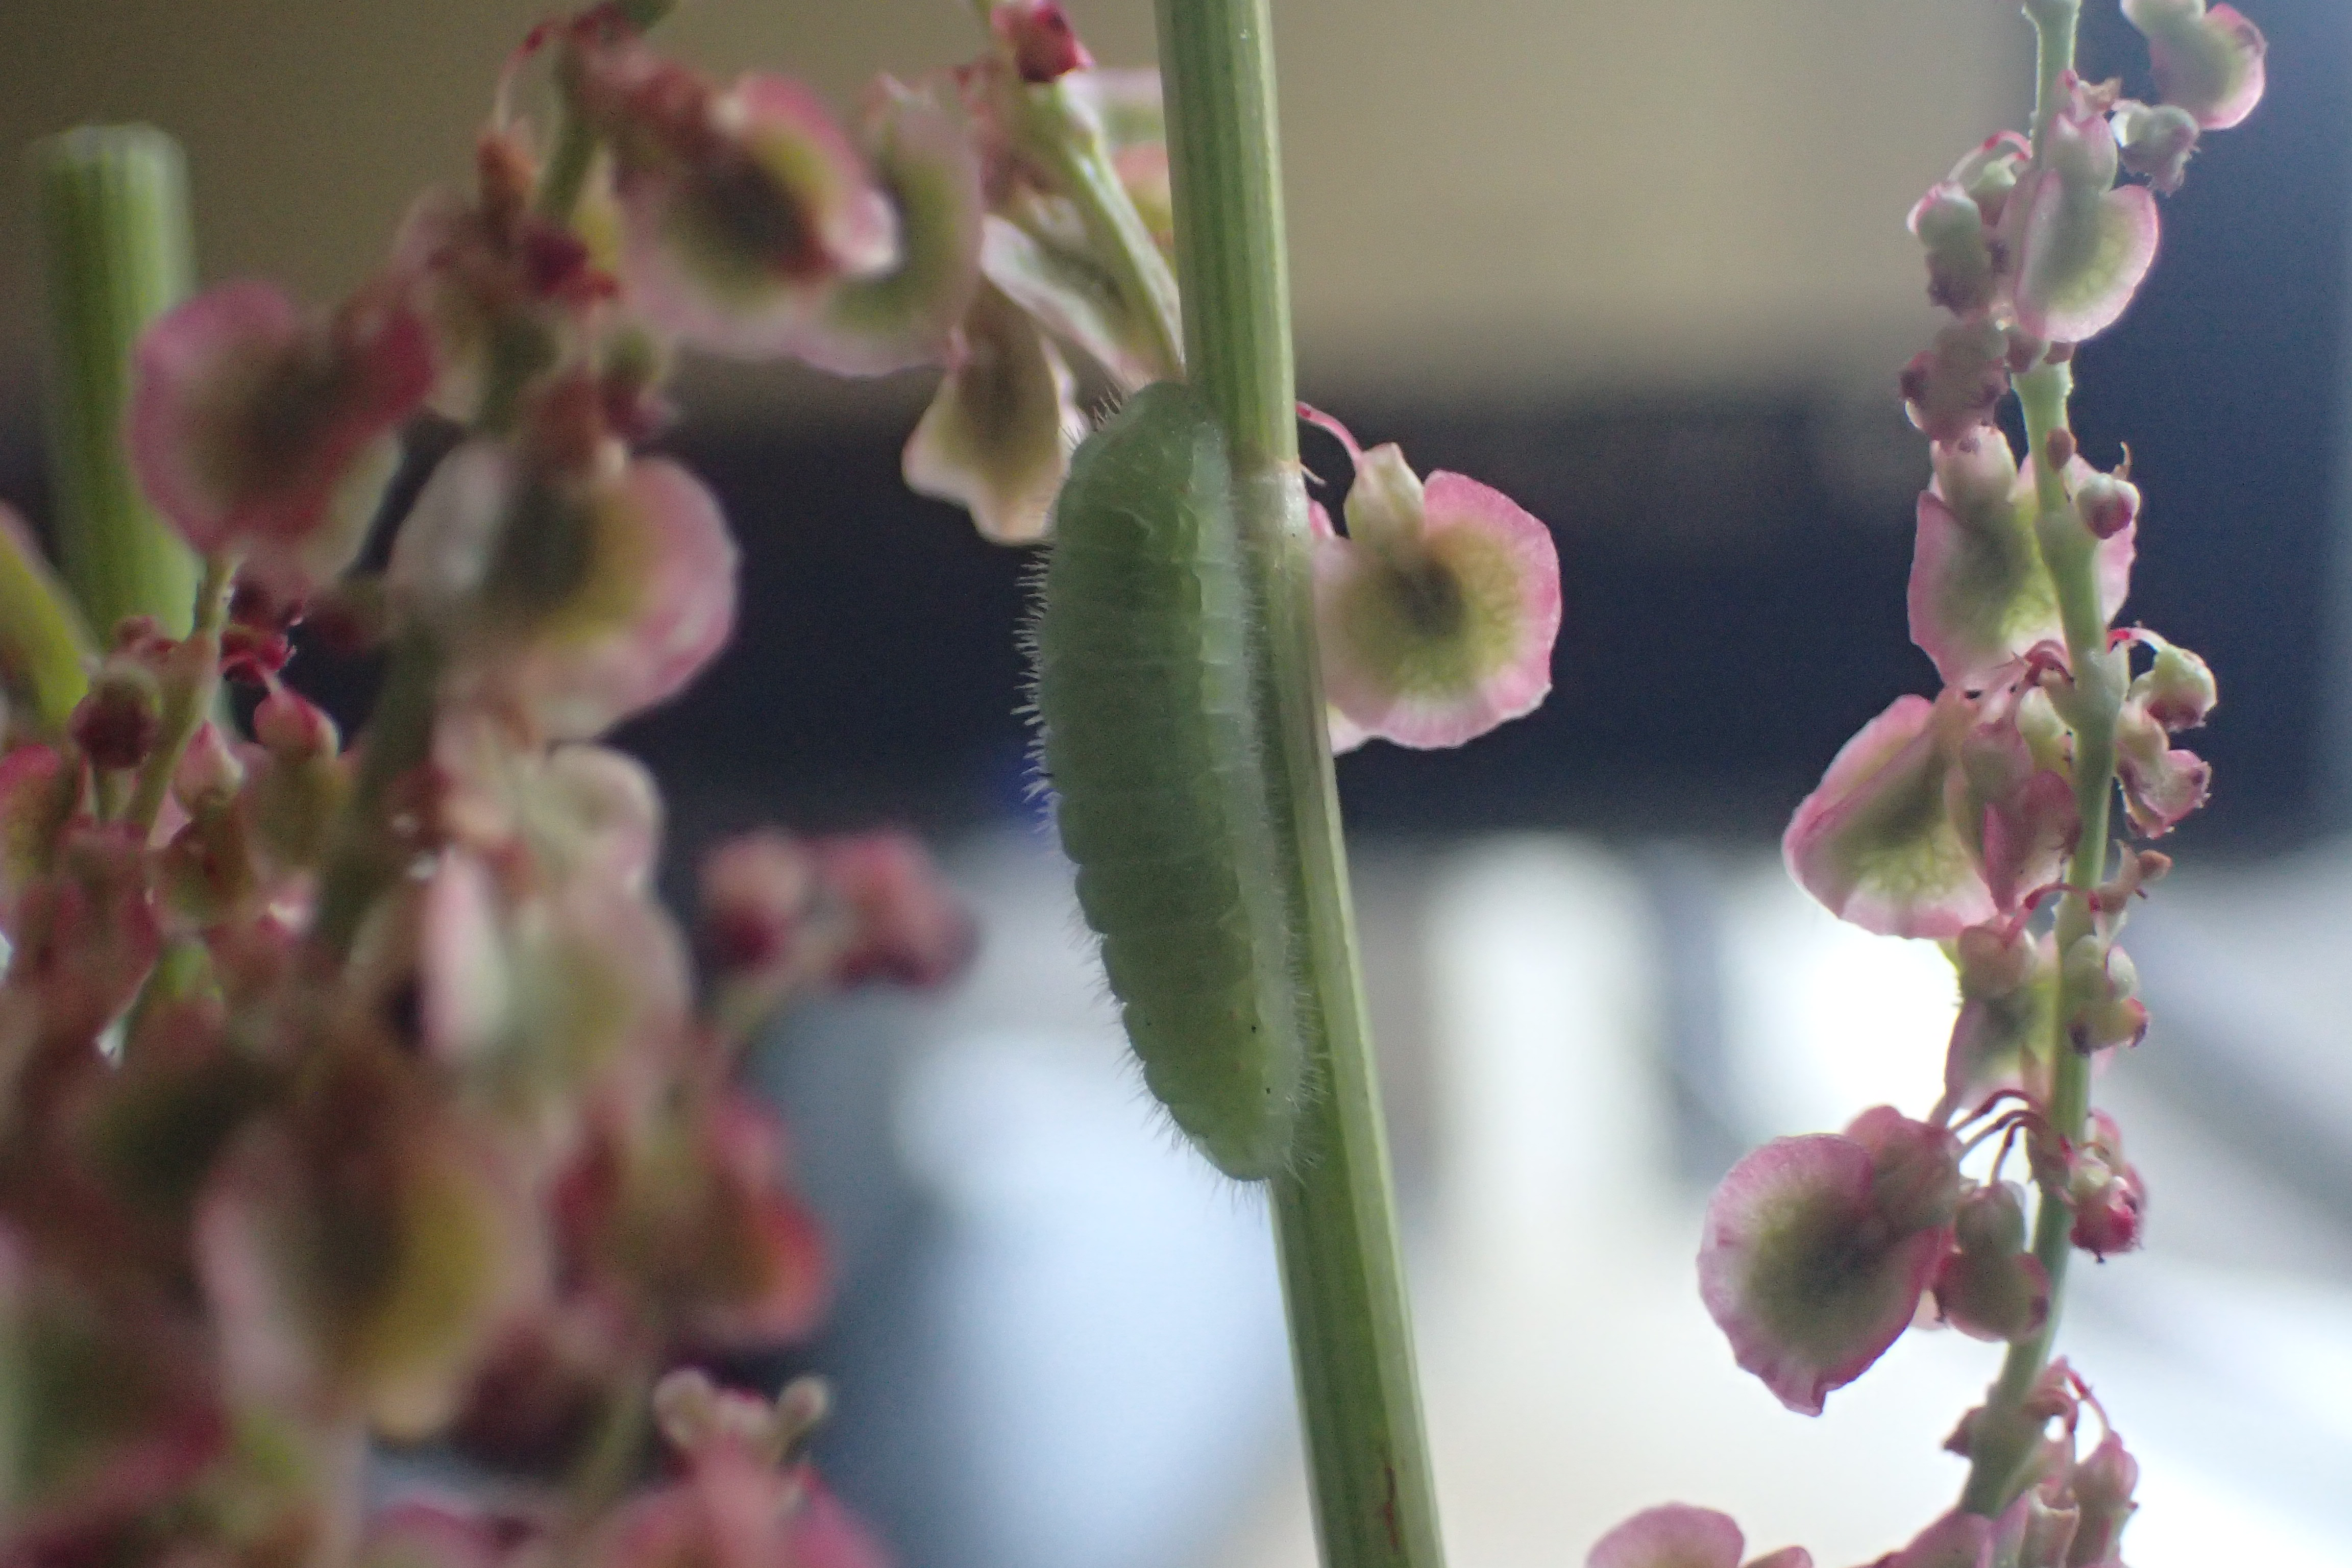
\includegraphics[width=5cm]{photo/sitting_on_branch.JPG}
    \caption{スイバの枝で静止していた幼虫}
    \label{pic-sitting-on-branch}
  \end{center}
\end{figure}

同様なポイントを探したところ, すぐ2匹目が見つかった. 
写真\ref{pic-field}のような, 割とひらけた場所であっさり見つかるようだ. 
\begin{figure}[htbp]
  \begin{center}
    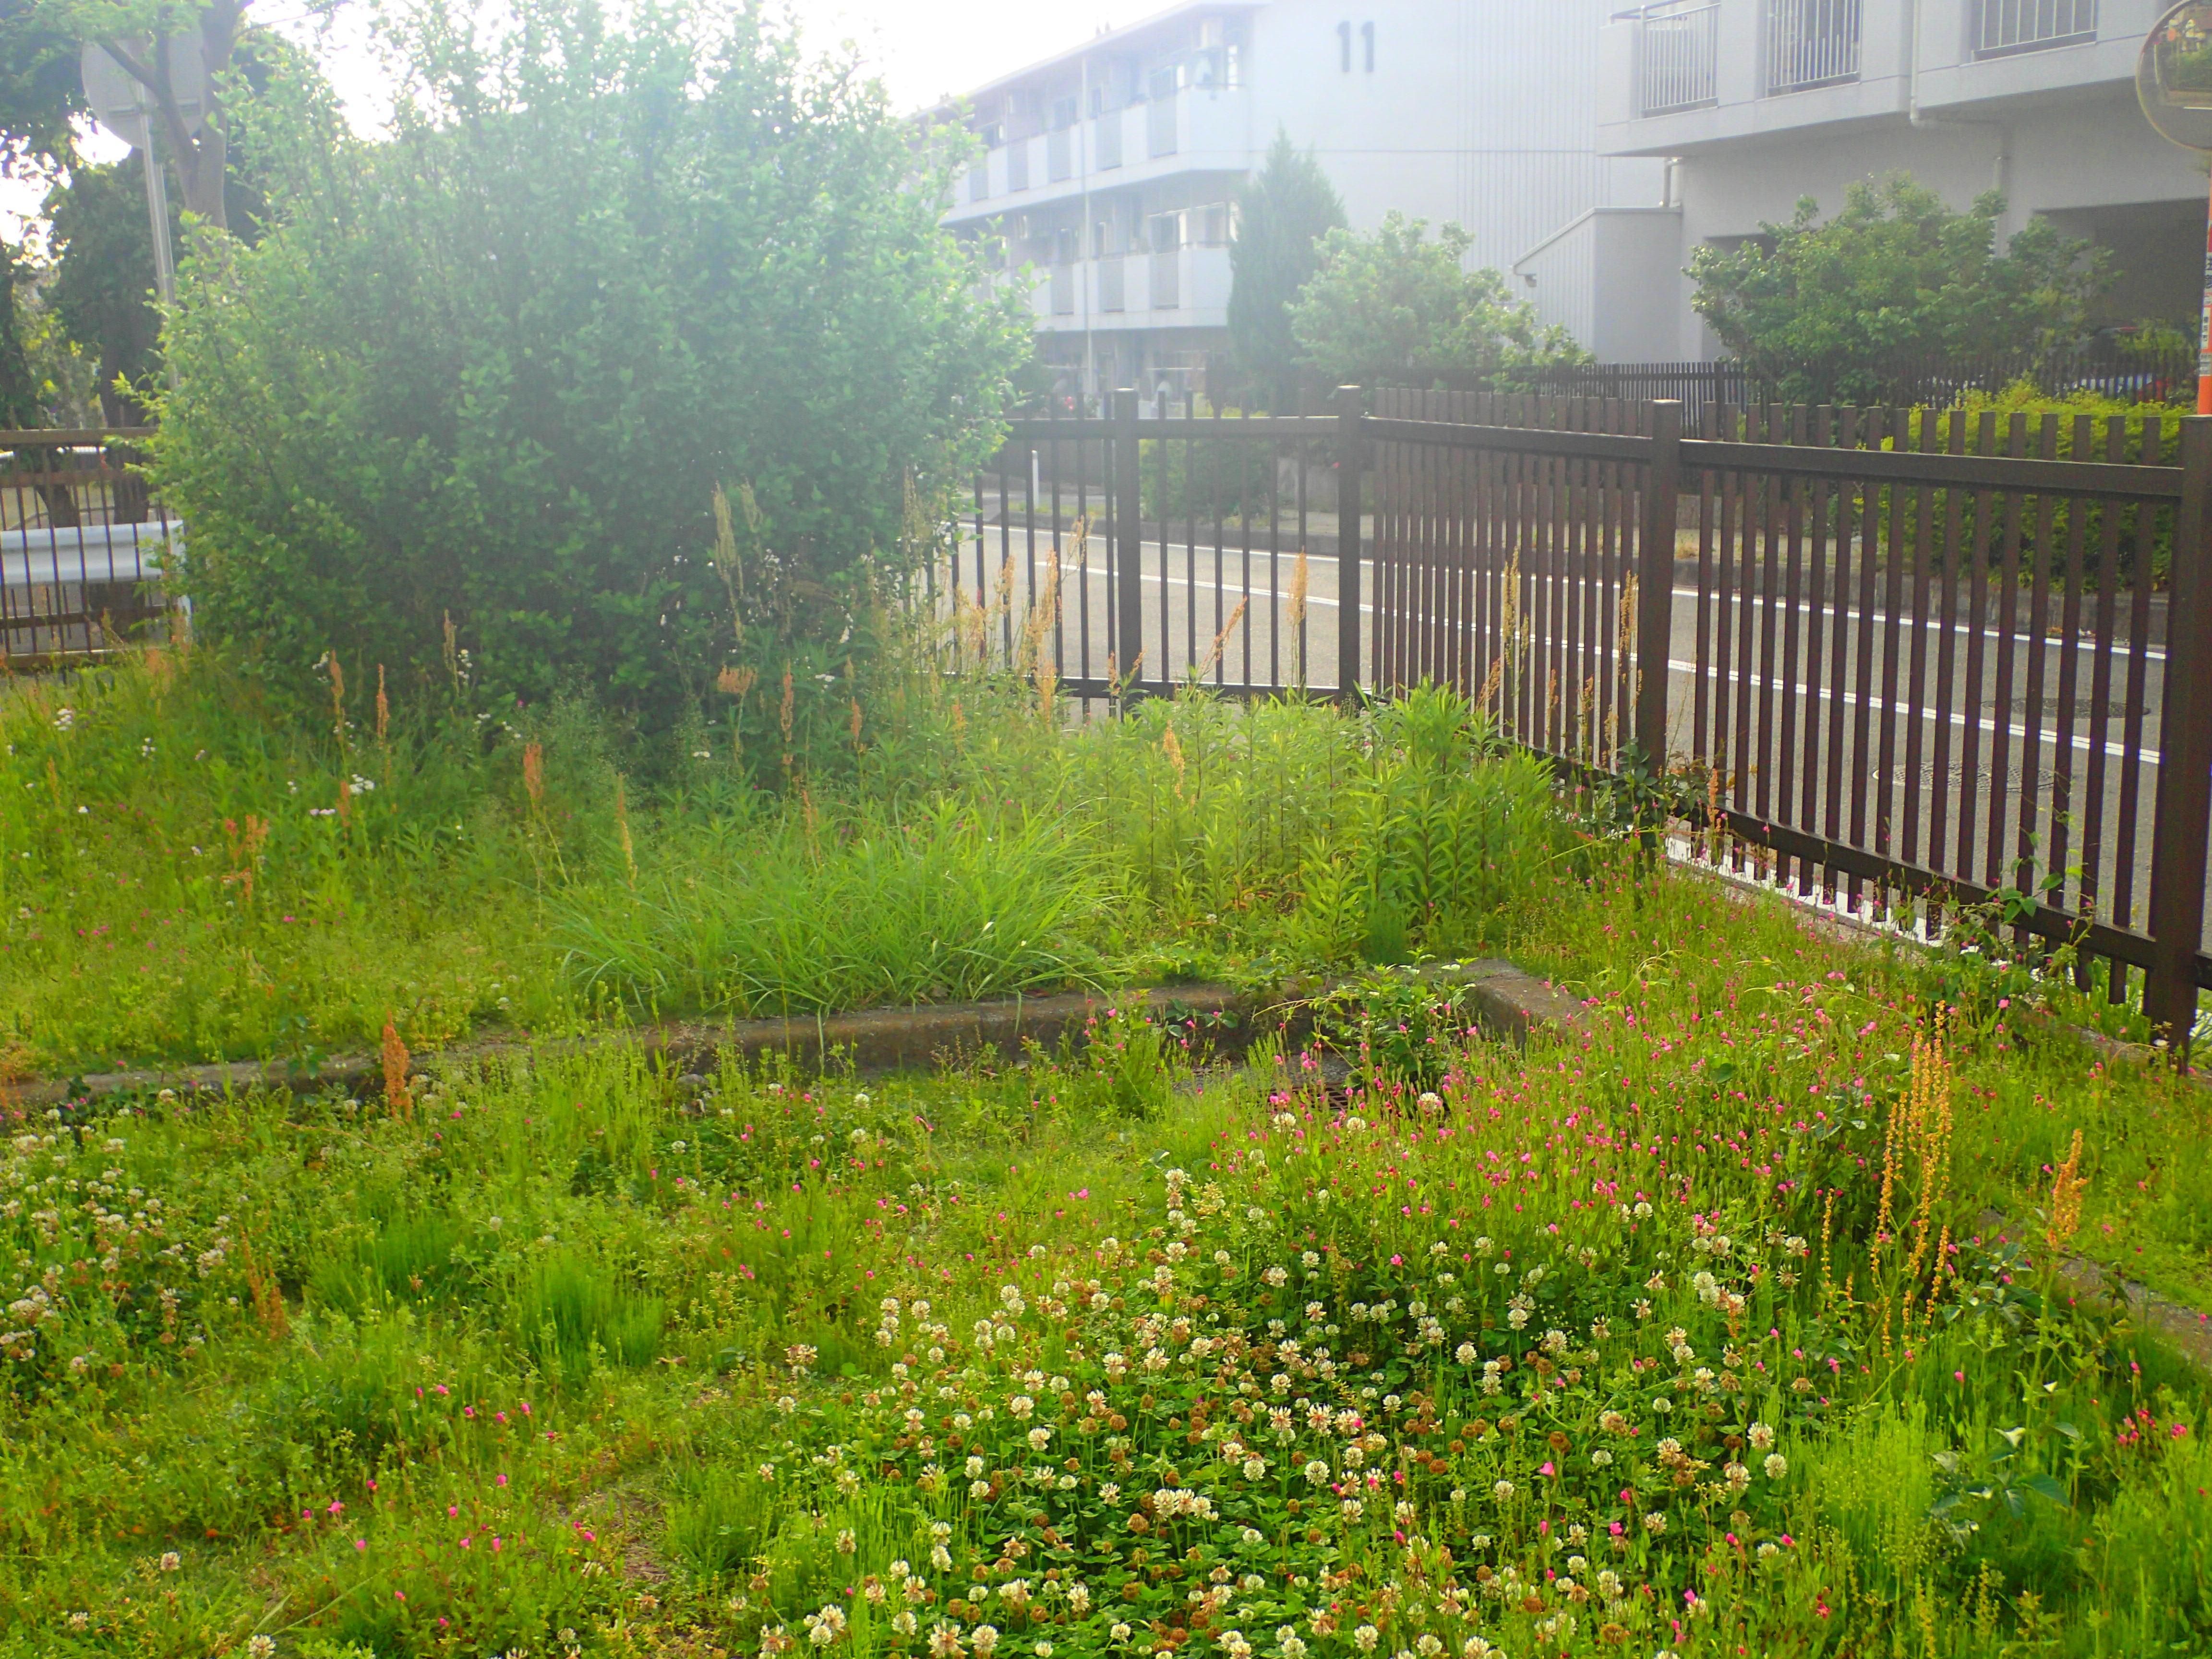
\includegraphics[width=5cm]{photo/park.JPG}
  \end{center}
  \caption{幼虫を発見した公園}
  \label{pic-field}
\end{figure}
最初に見つけた幼虫は, 1cm以上のサイズで, 2匹目の幼虫も, 1cm 弱のサイズで, どちらも終齢か, 4齢程度の幼虫と思われる. 
この時期は, 発生サイクル的に, 終齢が多い可能性がある. また, 終齢の幼虫は, 葉裏より, 花を食する可能性がある. 

\subsection{16時半:飼育環境の構築}
まずは, 採集時のスイバが乾燥しないように, 水を満たしたケースにさしたところ, そのわずかな振動で, 幼虫がぽろっと落ちた. 
その後, 幼虫は花によじ登ろうとしているように見えたが, 素直によじ登るというよりも, 頭を振りながら身をよじる動作をしていた. その動作のせいか, 登りかけては落ちるのを繰り返していた. 
脚で食草にしがみつく力は, アゲハ属の幼虫に比べると, 極端に弱いと推測される. 
また, それゆえに, 糸を吐き, 足場を作ろうとして, 妙な動作をしていたのではないかと推測される. 
\begin{figure}[htbp]
  \begin{center}
    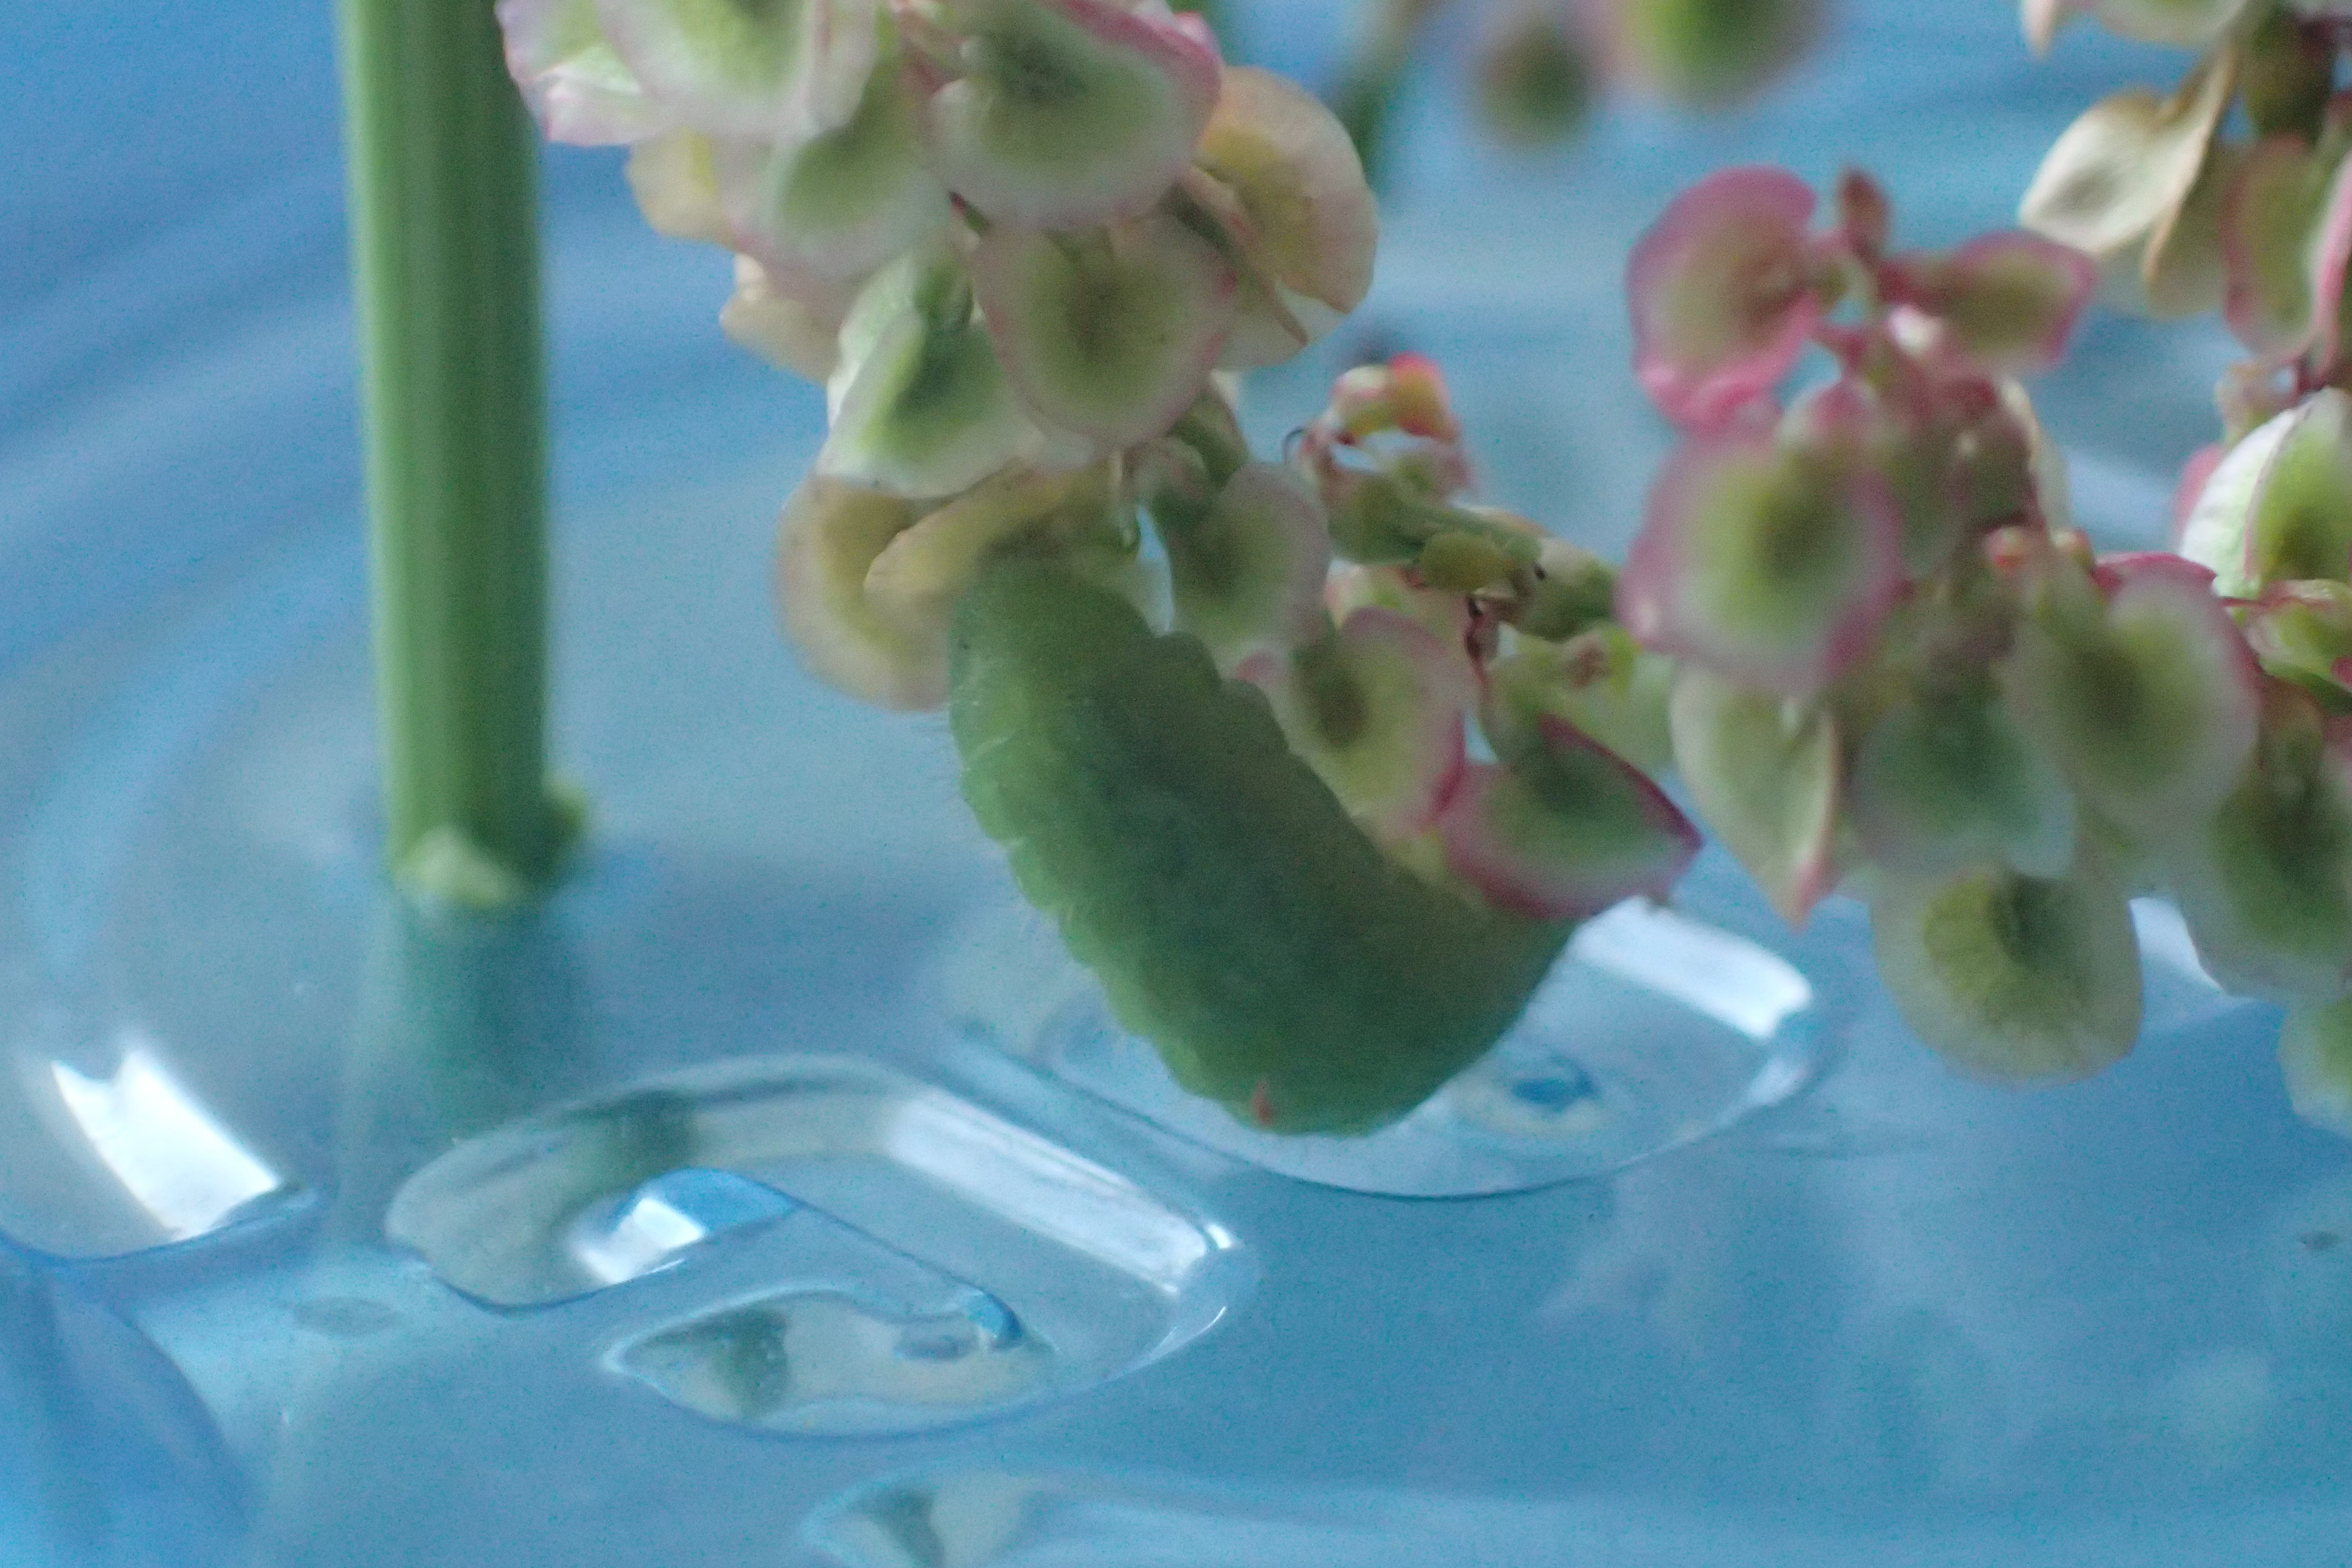
\includegraphics[width=5cm]{photo/try_to_climb.JPG}
    \caption{スイバの花によじ登ろうとする幼虫}
    \label{pic-try-to-climb}
  \end{center}
\end{figure}

\subsection{17時:飼育ケージの変更}
本来であれば, 自然界と同じように, スイバの花が垂直に上に伸びている状況を再現した方がよいと考えたが, 
枝から落下した幼虫があまりにも枝に戻ることができないのと, 世間のベニシジミ飼育のブログなどで, 枝を寝かせた状態で飼育しているものがほとんどであることから, 
枝を寝かせる方向にした. 捨てる予定であった, ガラスの耐熱ボウルを綺麗に洗浄し, スイバの枝に, 湿らせたキッチンペーパーを被せ, 
その上からアルミホイルでくるみ, 写真\ref{pic-environment}のような状況にした. 
\begin{figure}[htbp]
  \begin{center}
    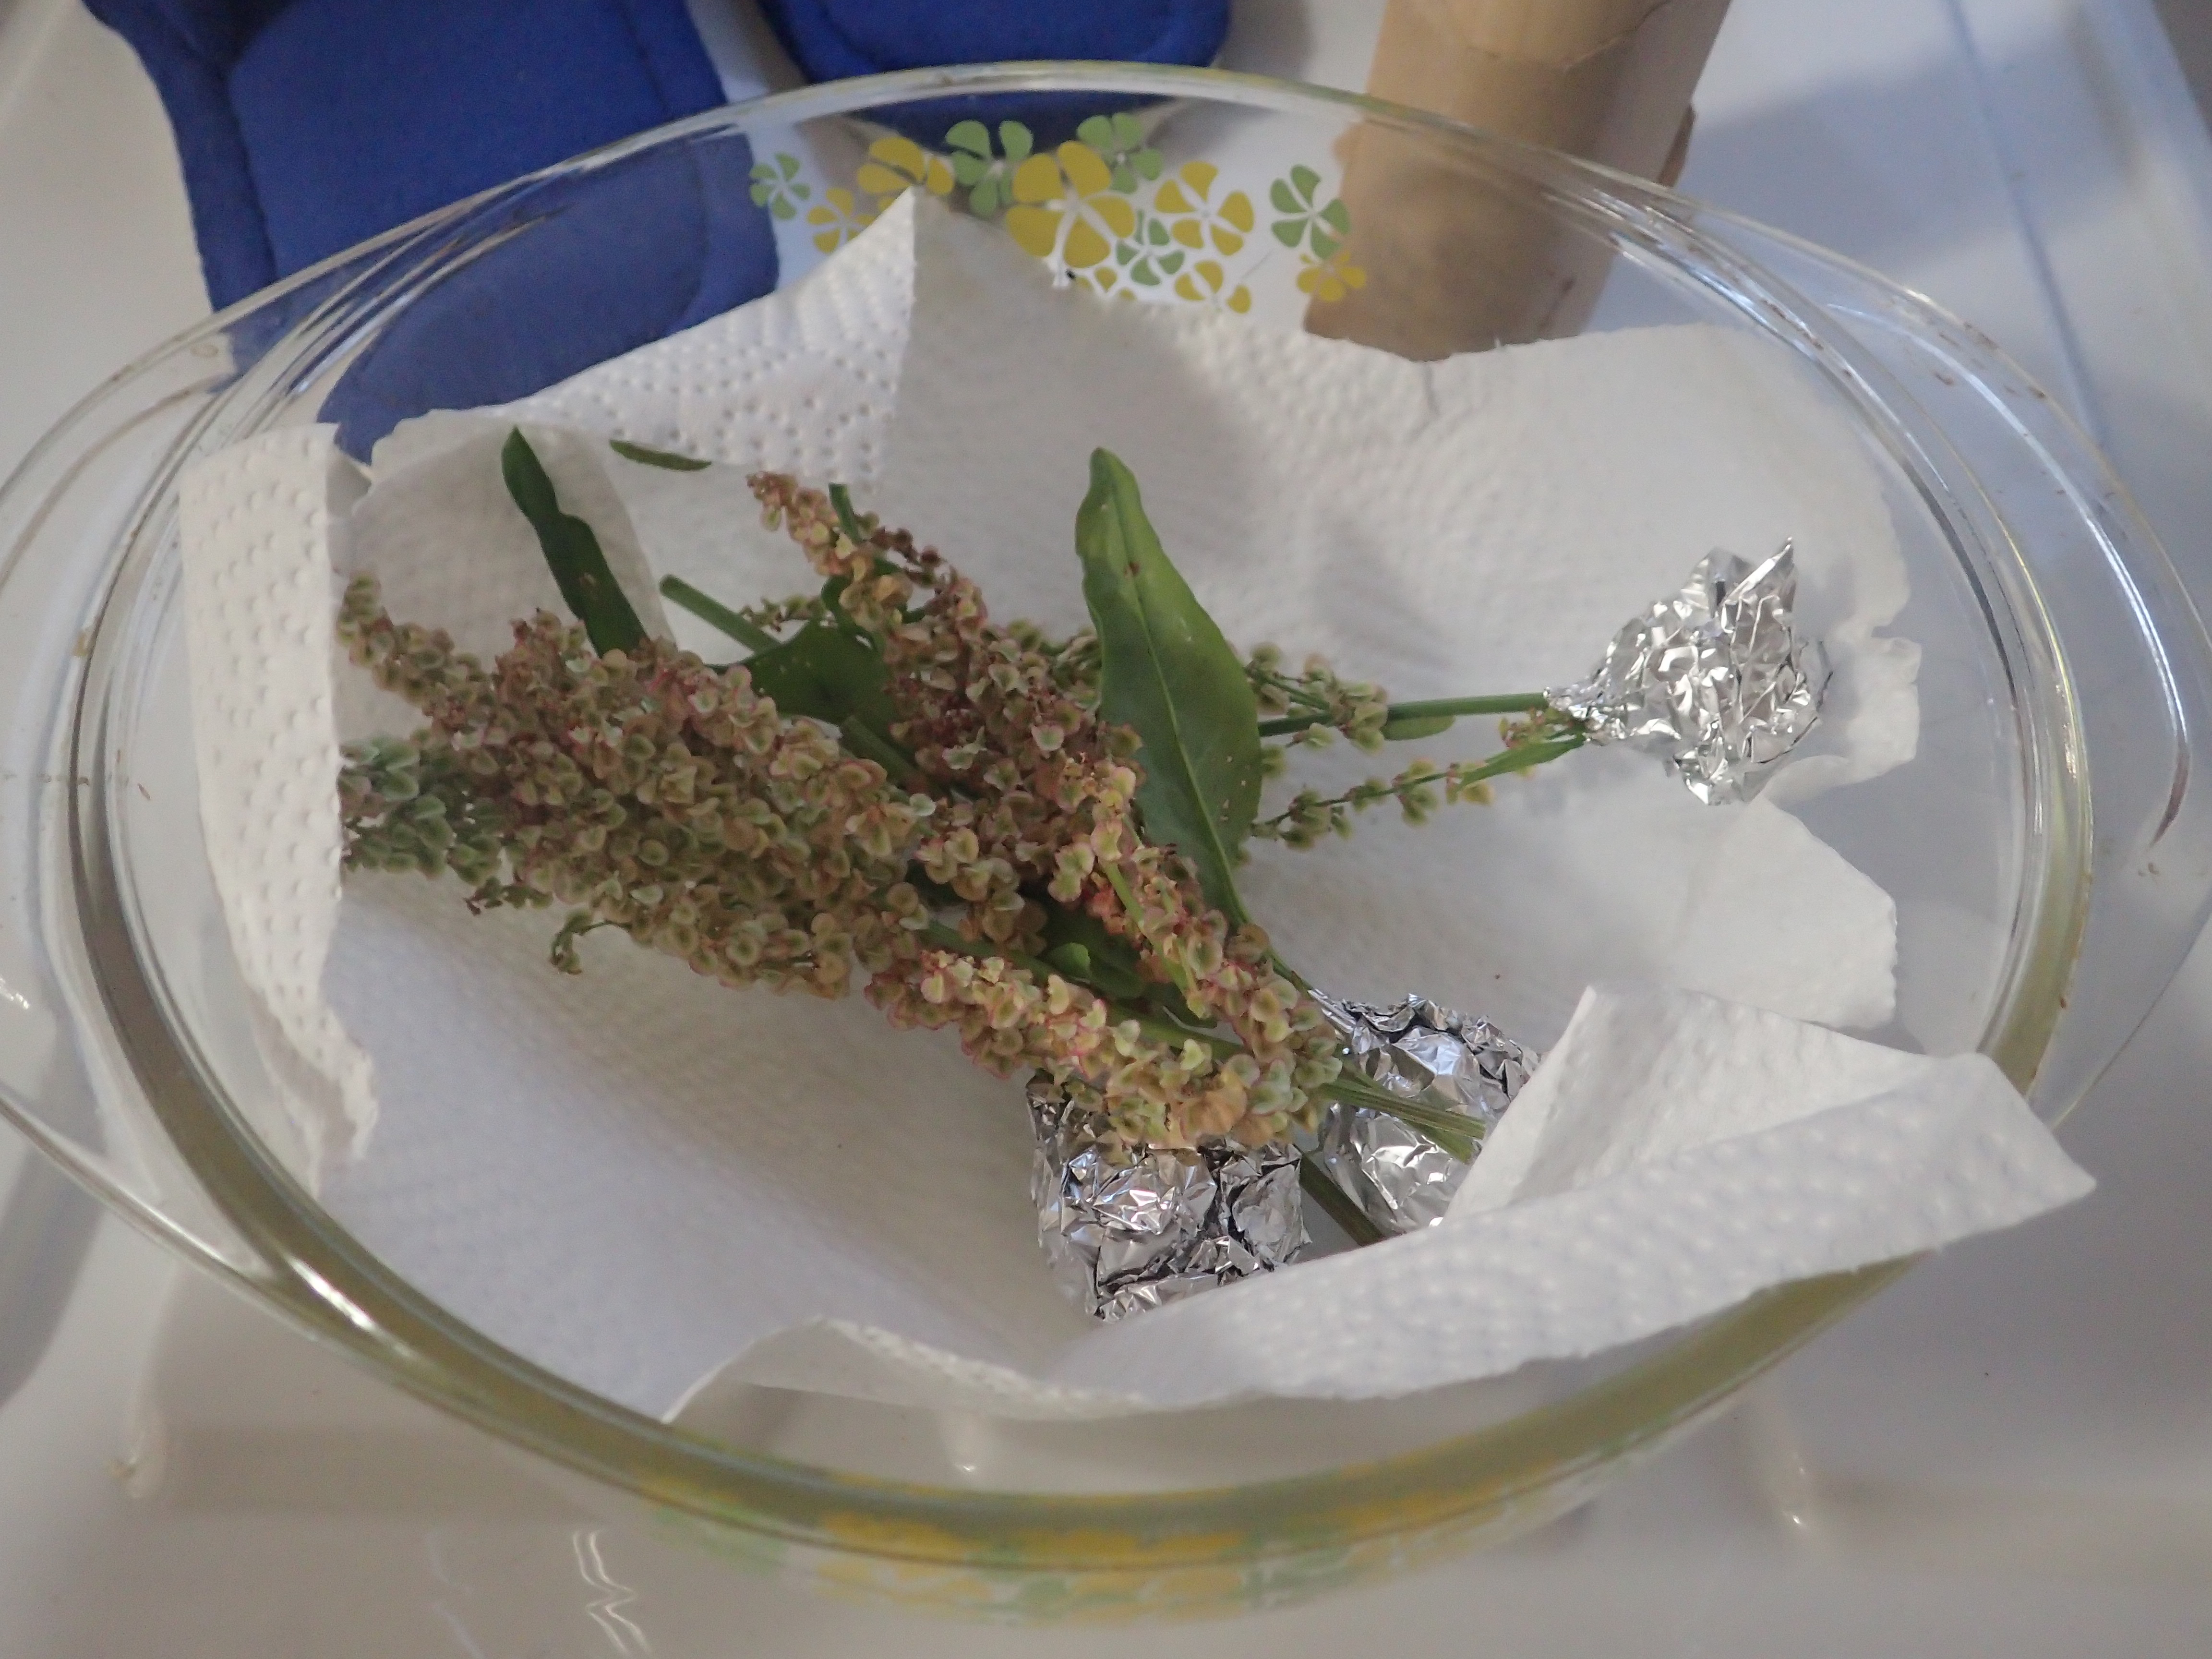
\includegraphics[width=5cm]{photo/environment.JPG}
    \caption{ガラスボウルによる飼育環境}
    \label{pic-environment}
  \end{center}
\end{figure}
また, ガラスボウルの底に, どうしてもスイバから漏れた水がたまり, 幼虫の溺死の危険があるため, 
底にはキッチンペーパーを敷いた. さすがの幼虫も, キッチンペーパーならば足が滑らないのか, 歩きやすそうに動いていた. 
その後, まだ外が少し明るかったので, 太陽光の代わりに, 爬虫類用のUVBランプに日没までの30分程度当てた. 
日本の環境にしては少し紫外線量が多いように思われたが, ガラス越しなので, 半減しているはずで, 問題はないと思われる. 

\subsection{18時:幼虫の移動}
食草の上を移動していた幼虫が, 2匹ともキッチンペーパーに降り, 移動を始めた. 
どこに移動するか見ていると, 写真\ref{pic-environment}の左上(よく見ると紙の裏から体がはみ出している)ように, やたらと紙の裏, 折れ曲がったところなどに移動して, そこで静止する様子が見られた. 
おそらく, 休む時は, 葉などの裏に隠れる習性からの行動であろうと思われる. 

\subsection{20時:活動の再開}
キッチンペーパーの裏でそのまま静止して翌朝まで寝てしまうのかと思ったが, 1時間程度しか静止しておらず, また移動し, 食草を食べている様子が確認できた. 
おそらく, 夜間でも, 短時間の休息と移動を繰り返すことで, 天敵に見つかる可能性を下げているのであろうと思われる. 
人間や, 犬猫と違い, 夜間にずっと寝ている, ということは無いようだ. 

\subsection{23時:糞の観察}
糞は, やや明るめの焦げ茶色で, 1mm程度の樽型のものが10個ほど確認できた. 

\newpage
\section{5/12の記録}
\subsection{9時:特に異常なし}
思いの外大量の糞をしていたので, 古い食草を捨てるとともに, 掃除. 
昨日, 枝に登るのに苦労していた個体も, しっかり枝に捕まって静止していた. 
寸法を測定したところ, どちらも15mm*5mm程度で, 思ったより寸法差はなかった. 
葉が食われていたが, 表面だけを舐めるような食痕ではなく, 写真\ref{Larba-day2-2}のように, アゲハのような食痕であった. 
他のブログなどと矛盾するが, 与えている葉が, 柔らかい若い葉であることが要因なのかもしれない. 

\begin{figure}[htbp]
  \begin{minipage}{0.5\hsize}
    \begin{center}
      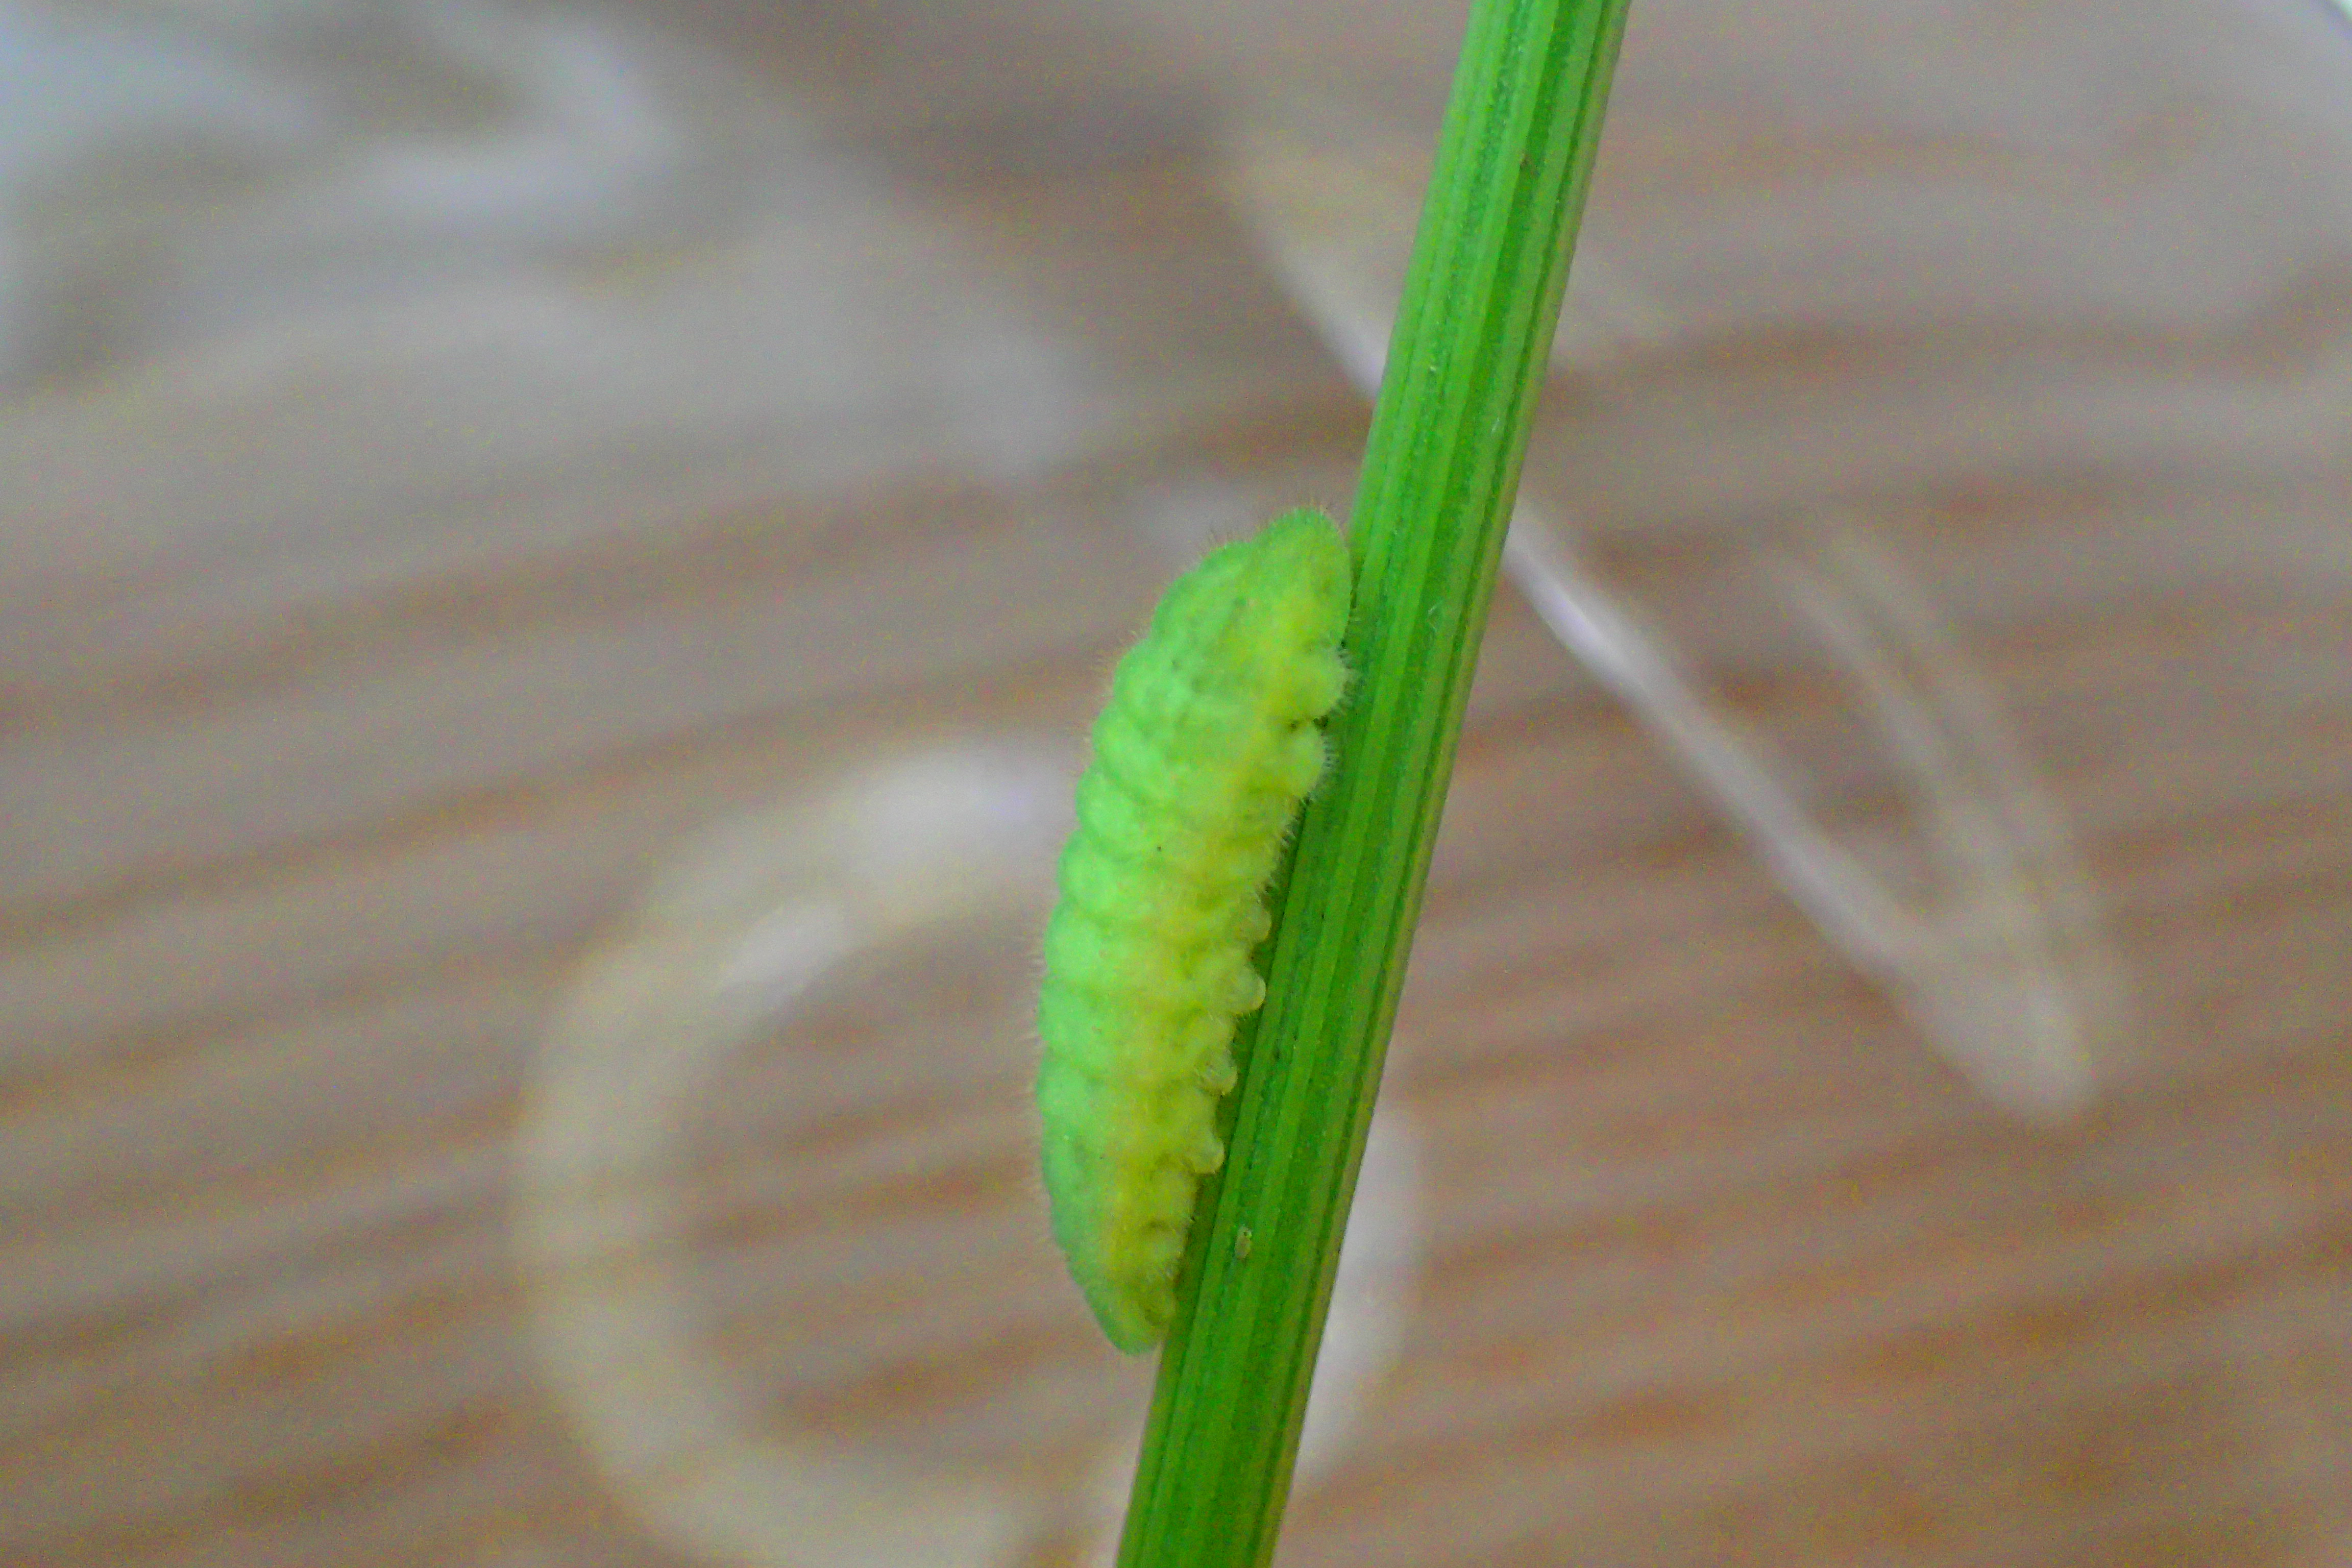
\includegraphics[width=5cm]{photo2/Larva1.JPG}
    \end{center}
    \caption{幼虫1の状態}
    \label{Larba-day2-1}
  \end{minipage}
  \begin{minipage}{0.5\hsize}
    \begin{center}
      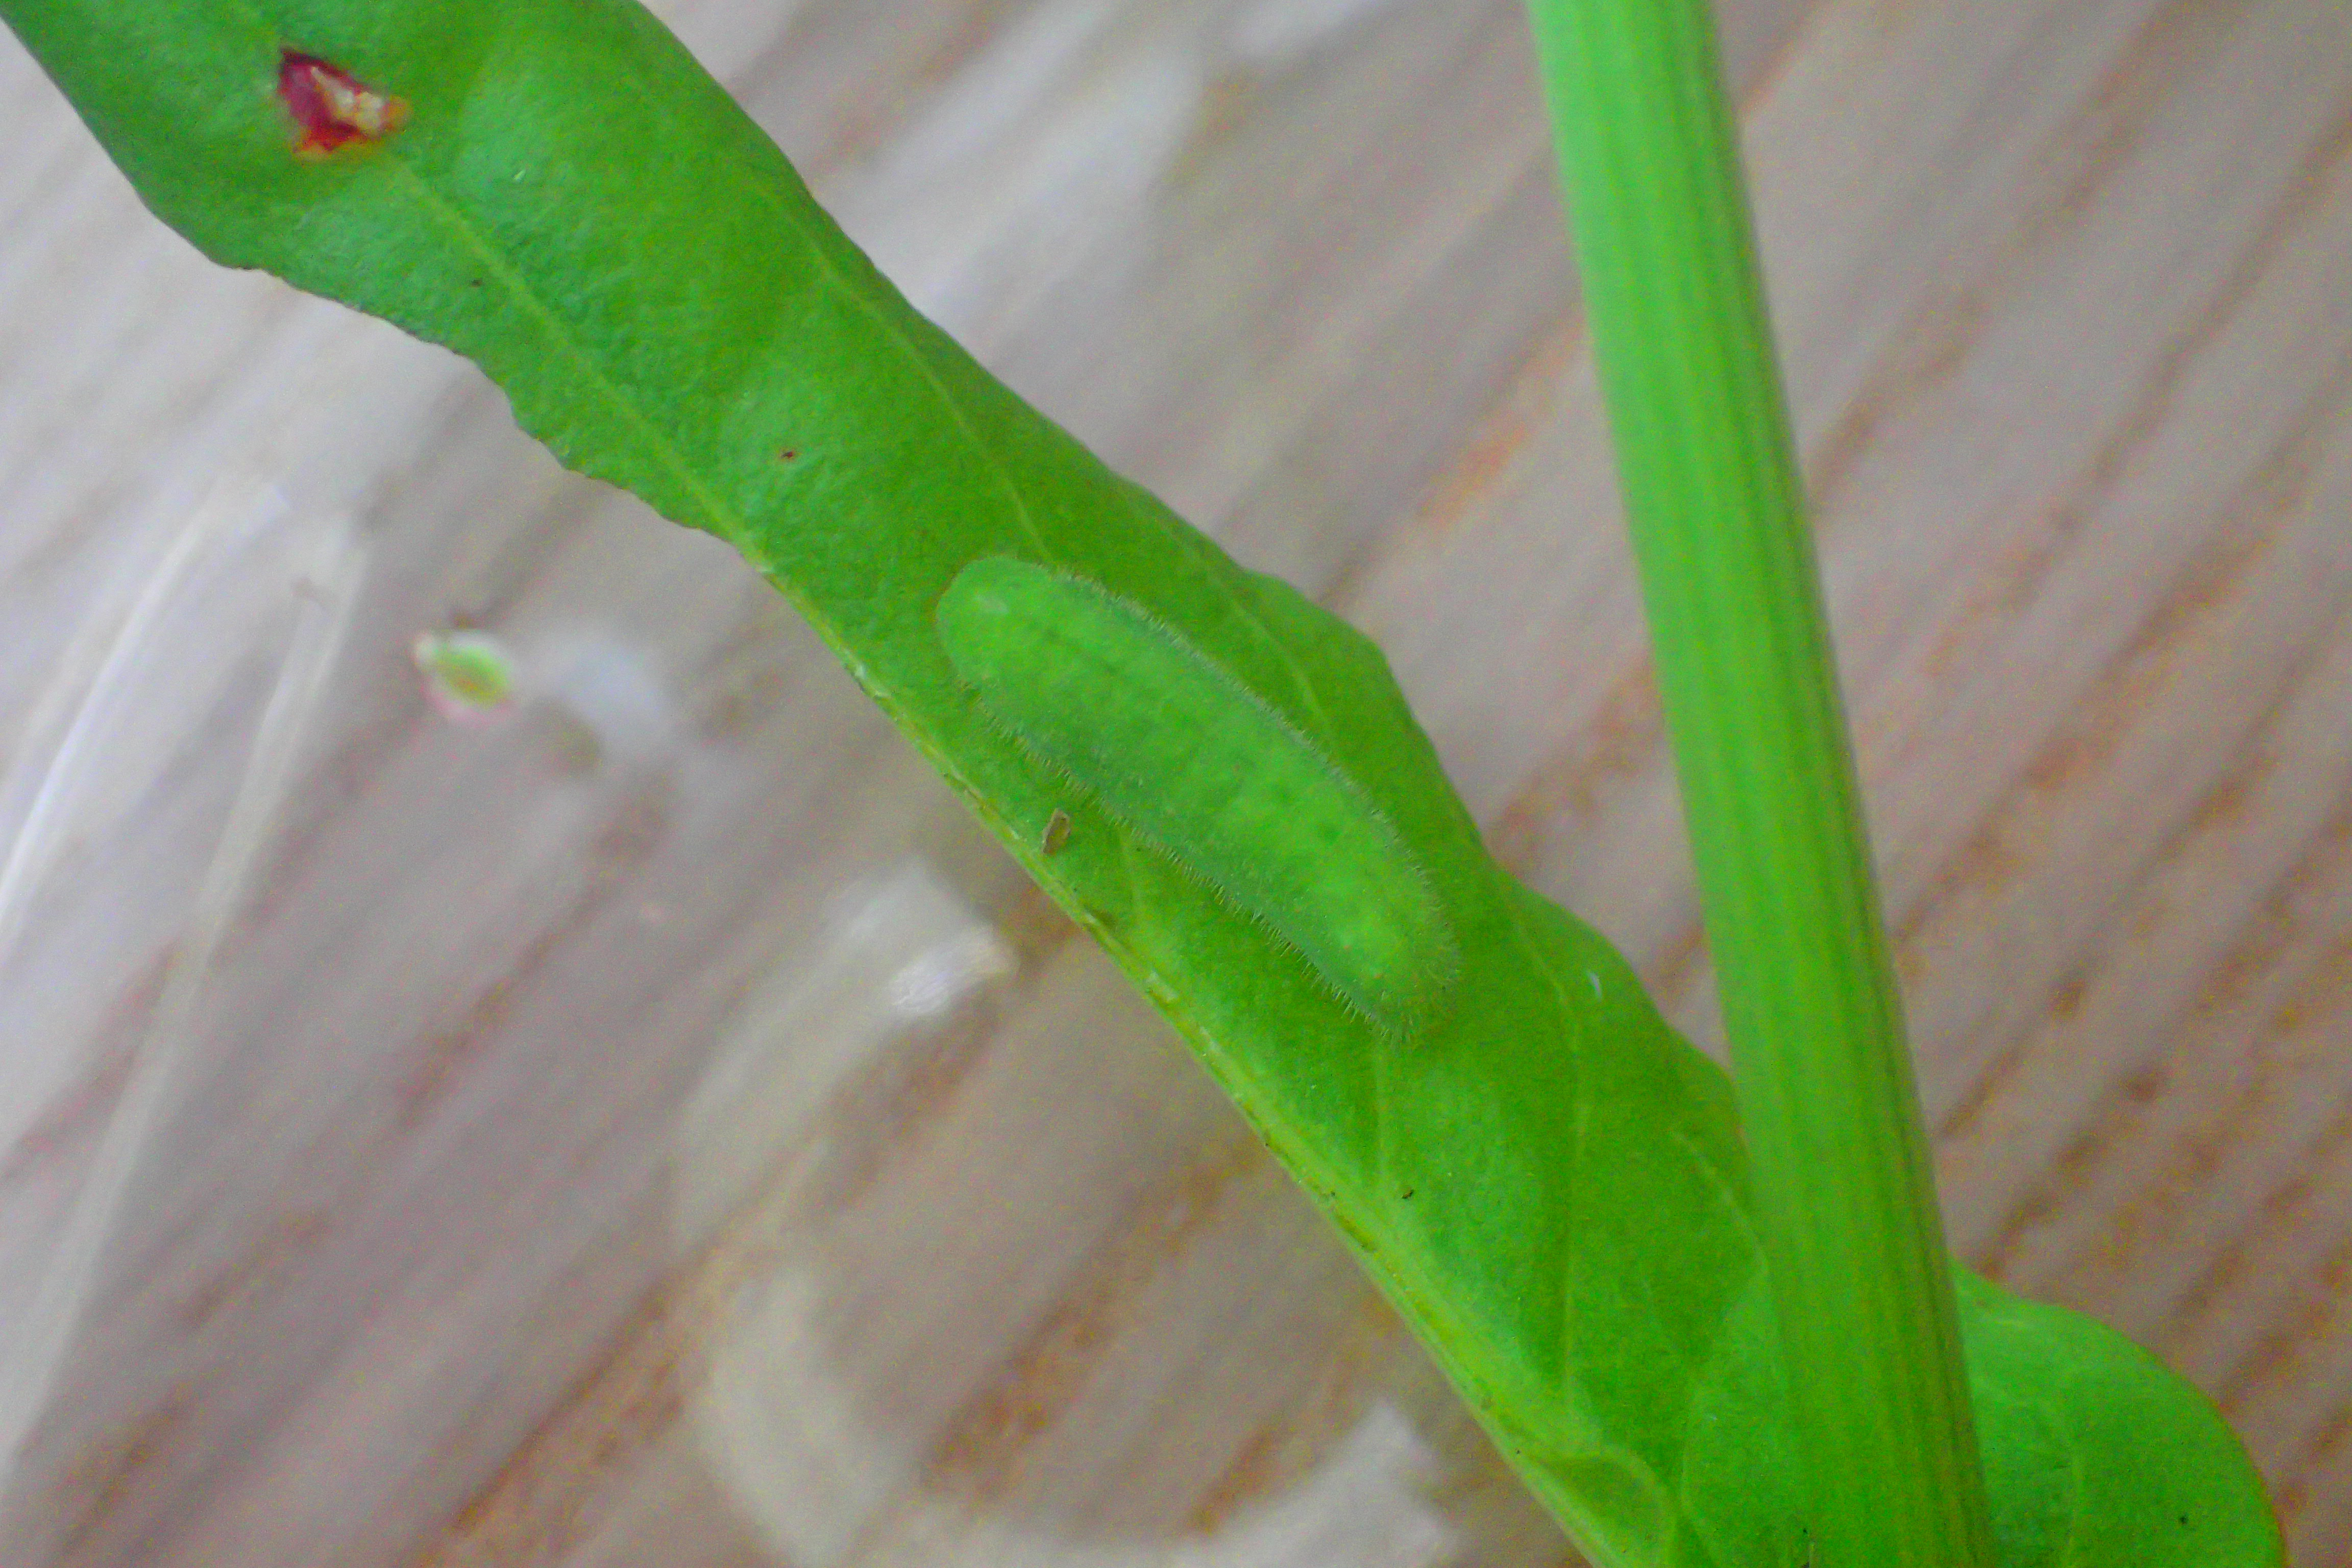
\includegraphics[width=5cm]{photo2/Larva2.JPG}
    \end{center}
    \caption{幼虫2の状態}
    \label{Larba-day2-2}
  \end{minipage}
\end{figure}

\subsection{15時:餌の採取と幼虫の居場所}
幼虫の採集場所と同じところに, 新しい餌用のスイバを取りに行ったついでに, 
幼虫を探した. 簡単に, 同じ苗で2匹見つかったが, やはりどちらも, 花に近いところの枝, 花の中で見つかった. 
やはり, 幼虫はあまり葉にいないのだろうか. 
家に帰り, ケージ内の幼虫がどこにいるか見たところ, 2匹とも花を避け, 葉の上にべったりとくっついていた. 
単純に花, 葉というより, 鉛直方向に上を目指す傾向があるだけなのか. 
よくわからない. 

\subsection{16時:鶴見川堤防のギシギシで幼虫を探す}
会社に行く用事を済ませたのち, 鶴見川沿いの堤防に群生するギシギシに幼虫がいないか探してみた. 
鶴見川の堤防は, 写真\ref{pic-Tsurumi-River}のような, ギシギシの群生があちこちに見られ, ベニシジミの食草は豊富である. 
\begin{figure}[htbp]
  \begin{center}
    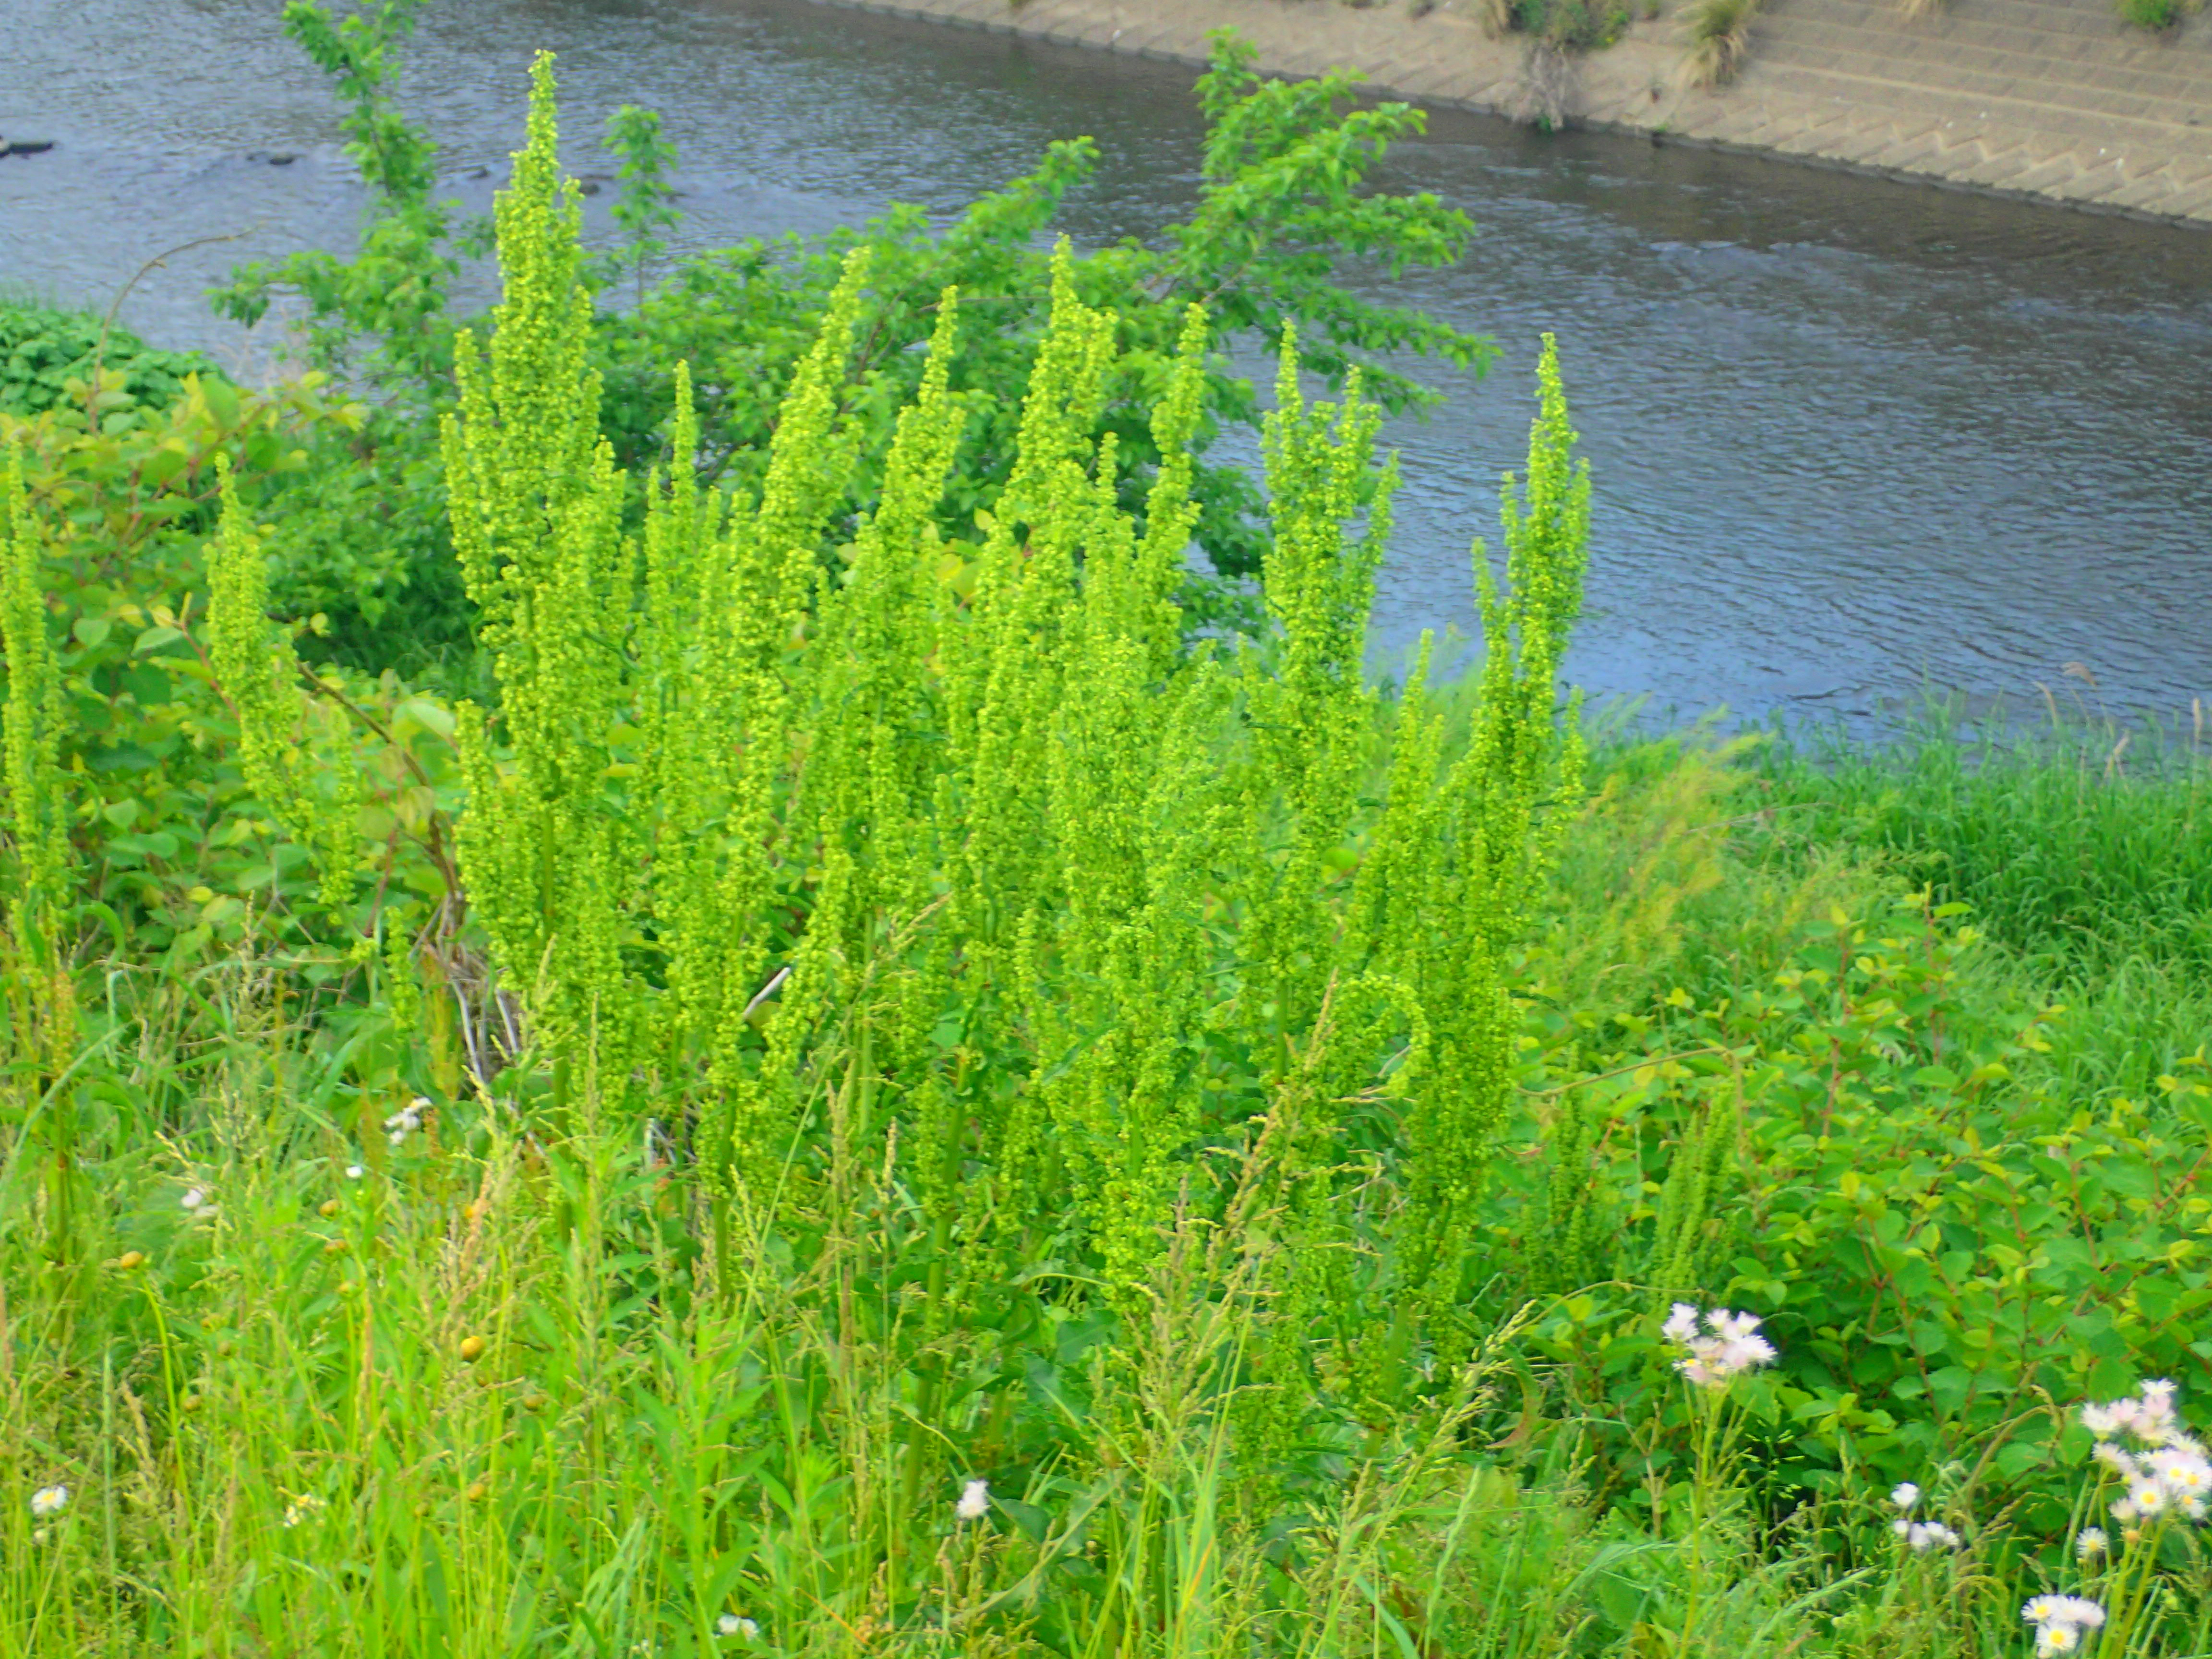
\includegraphics[width=5cm]{photo2/TsurumiRiver.JPG}
  \end{center}
  \caption{ギシギシの群生}
  \label{pic-Tsurumi-River}
\end{figure}
また, 定期的な草刈りこそはいるものの, 自然環境としては良好で, 様々な植物が生えている. 
ところが, 公園ではあっさり見つかった幼虫が, どれだけ探しても見つからなかった. 
ハグロハバチの幼虫ですら, 見つかりはしたが, 公園と比べると極端に数が少なかった. 
理由はわからないが, 状況証拠として, 
\begin{itemize}
  \item 鶴見川の堤防は, スイバも存在するが, ギシギシが極端に多い
  \item 鶴見川の堤防は, ギシギシ, スイバ以外に, 背の高い植物が多い
  \item 鶴見川の堤防は, いつも割と強い風が吹いている
\end{itemize}
というような環境要因があり, どうもベニシジミは, ギシギシよりはスイバを好み, 割とひらけていて草がまばらな, 風のそれほど強くない環境を好むのかもしれない. 
特に, 風については, ベニシジミ幼虫の, しがみつく力の弱さからすると嫌がりそうな気がする. 
また, ギシギシの葉は, スイバの葉よりも明らかに固そうで, 幼虫が食す上では, あまり好まれそうにない. 

\subsection{19時:特に異常なし}
糞の掃除, 餌の交換を実施. 相変わらず幼虫は葉の上にいる. 自然界と何が違うのか. 彼らが花に向かわない理由が, 
今の所, 苗が鉛直に立っているか否かしか想像できない. 
ついでに, 鶴見川堤防沿いの, ギシギシの葉も餌として追加してみた. 結局どちらの葉におちつくか楽しみだ. 

\section{5/13の記録}
\subsection{9時:特に異常なし}
餌を見たところ, ギシギシには全く食いついていなかった. 
やはりスイバの方が好きなよう.

\subsection{13時:幼虫にダメージを与えてしまったか}
朝から, 日光に当てる目的で, 外にケースを出していたが, 
ガラスボウルの特性により, 中に熱気がこもり, サウナ状態になっていた. 
スイバはしおれ, 幼虫も何やら元気がない. 

\subsection{19時:幼虫のダメージは深刻かもしれない}
幼虫が, 動いてはいるものの, やたら体を丸めたり捻ったりして, 体勢がおかしいのと, 餌をあまり食っていない. 
ふんが, 下痢のようになっている. 葉に戻しても, すぐ丸まってひっくり返る. ちょっとまずい. 

\subsection{23時:とりあえず体勢はおちついている}
体勢は水平なまま落ち着いているが, 餌をくったり糞をした形跡がない. 体液なのか, 下痢なのかわからないが, 
赤茶色いシミがあちこちにある. とりあえず明日から外に出すのはやめる. 

\section{5/14の記録}
\subsection{9時:もう死んでいるかも}
まったく動かず, 餌も食べていない. 糞の排出もない. 赤茶色の汁も少し出ている. 
もうダメかもしれない. 高熱のダメージがよほど大きかったか. 

\subsection{16時:追加の2匹を捕獲}
新しく2匹を捕獲した. サイズ感からすると, 3齢か4齢といったところ. 

\subsection{18時:まだ生きている}
餌を食わない, 糞を出さないことには変わりないが, 汁はでていない. 
死んでいると思われた2匹が, 非常に緩慢な動作ではあるものの, 移動をしている. 
餌を食わない時点で, 長くはないように思われるが, もしかすると持ち直すかもしれない. 要経過観察. 

\section{5/15の記録}
\subsection{10時:生きているが・・・}
相変わらず餌食い, 糞はない. 汁はもう出ていない.
もう死んだかと思っていたが, よ〜く目を凝らしていると, 少しだけ動いているのと, 
光を当てると反応して動く. 休眠という行為である可能性を信じたい. 
新しい2匹は相変わらず元気だが, 瀕死の2匹が元気だった頃と比べて, 葉に対する無関心さがひどい. 
同じ公園の中から, 比較的若くて食べやすそうな葉をチョイスしているのだが, もっぱら花ばかり食べている. 

\subsection{17時:餌の中に投下するも}
もとの2匹のうち, 大きい方は, もう全く動かない. 小さい方は, 目に見えるような動作こそないものの, 
しばらくほっとくと, なかなかの距離を移動しており, 明らかに生きている. しかし餌食い, 糞はない. 
こちらにも, 花を与え, 花の中においてやった. 
元気な2匹は, 新しい花を与えるとすぐそちらに移動して食い始めた. 彼らは心配なさそう. 

\subsection{22時:なぜ餌から離れようとする}
もとの2匹のうち, 大きい方はもう完全に移動がない. 小さい方はやはり移動こそするものの, なぜか食草から距離を取ろうとする. 
\begin{figure}[htbp]
  \begin{center}
    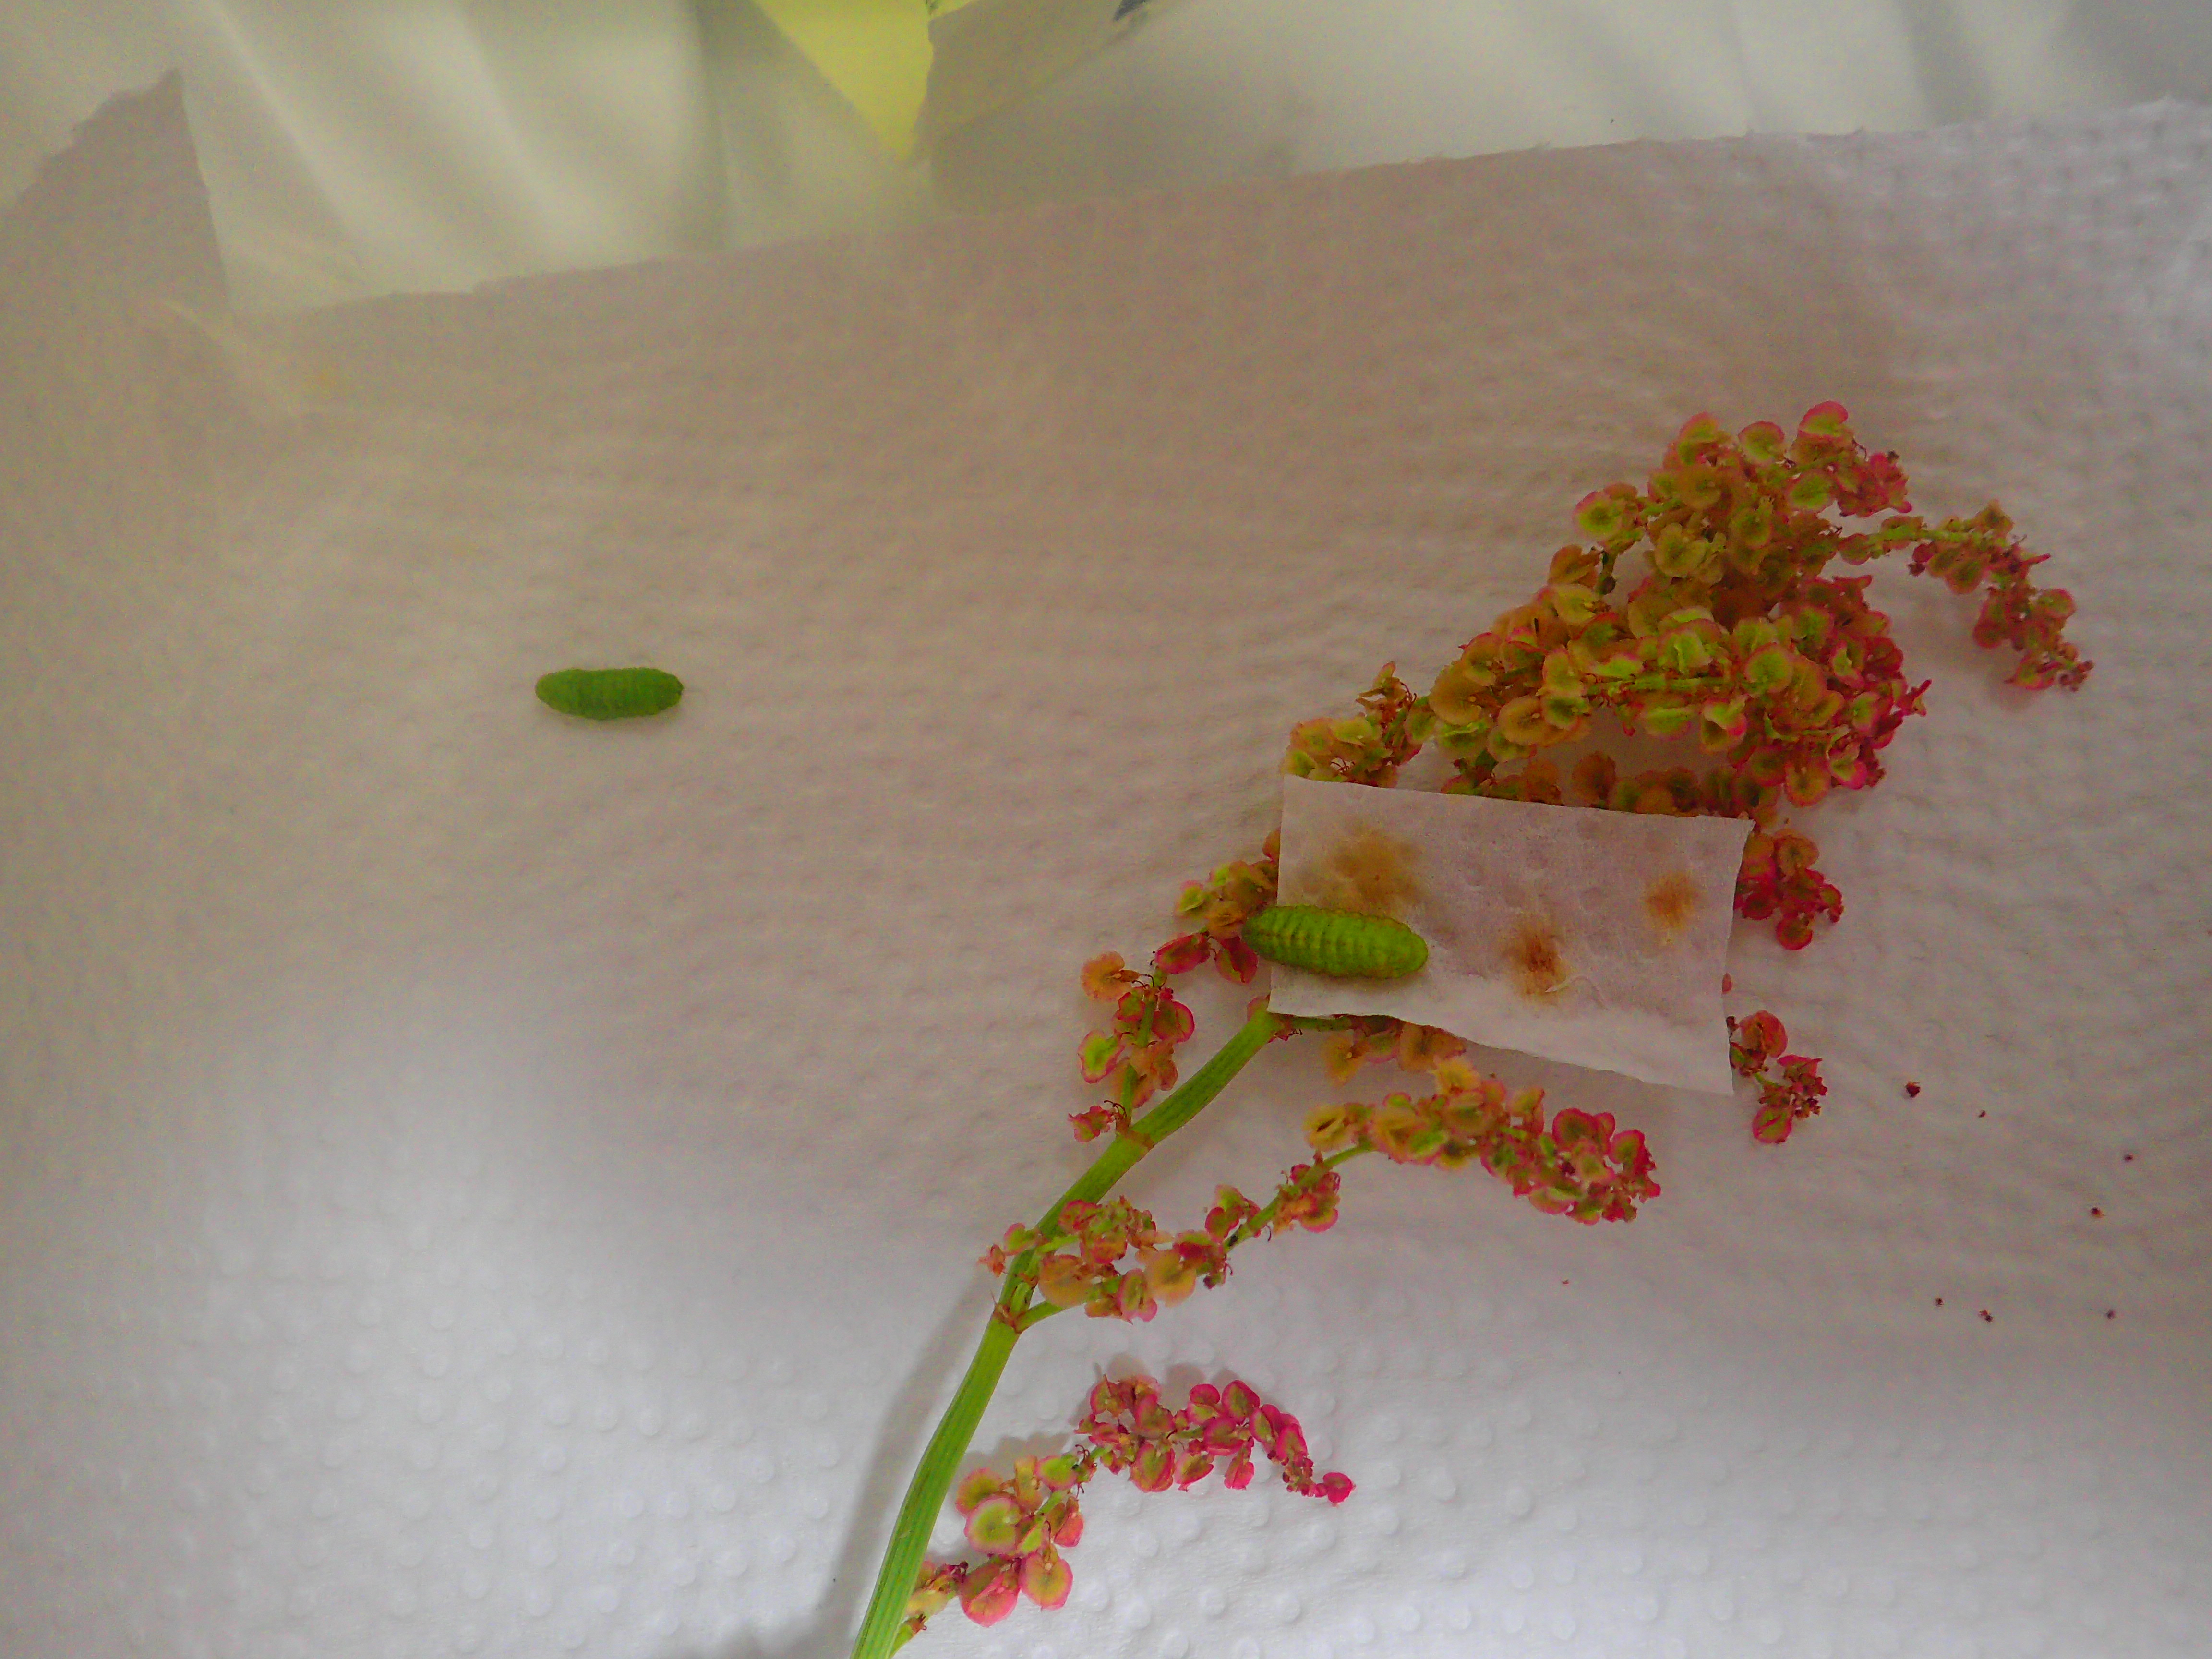
\includegraphics[width=5cm]{photo3/LarvaAwayFromFeed.JPG}
  \end{center}
  \caption{幼虫が食草から離れようとする}
  \label{pic-LarvaAwayFromFeed}
\end{figure}
この動作がなんなのかわからないが, 高熱で脳がやられたか, 何かの予兆かだろう. 
新しいやつらはあいかわらずもりもり食べている. この2匹は確実に蝶にしたい. 

\section{5/16の記録}
\subsection{10時:おそらく死んでいる}
2匹とも全く動かない. 大きい方は色も黒ずんできた. 明日判断しよう. 
小さい方も, 動きはない. もうダメだと思われる. 

\subsection{15時:蛹になるか}
元気な2匹のうち, 一匹が急にいなくなったと思ったら, キッチンペーパーの裏に移動した. 
何やら縮こまっているので, 前蛹と思われる. 意外と早かった. 

\subsection{22時:前蛹の様子がどうも変}
前蛹が, 異様に小さい. また, この状態に入ってから変化がなさすぎるのと, 変な色に変化してきた. 
具体的には黄色がかかっている. さらに, 片方だけに, 黒い大きな斑点が見られる. 
寄生されている可能性が高い. やはり野外で捕獲した幼虫はこんなものか. 
\begin{figure}[htbp]
  \begin{center}
    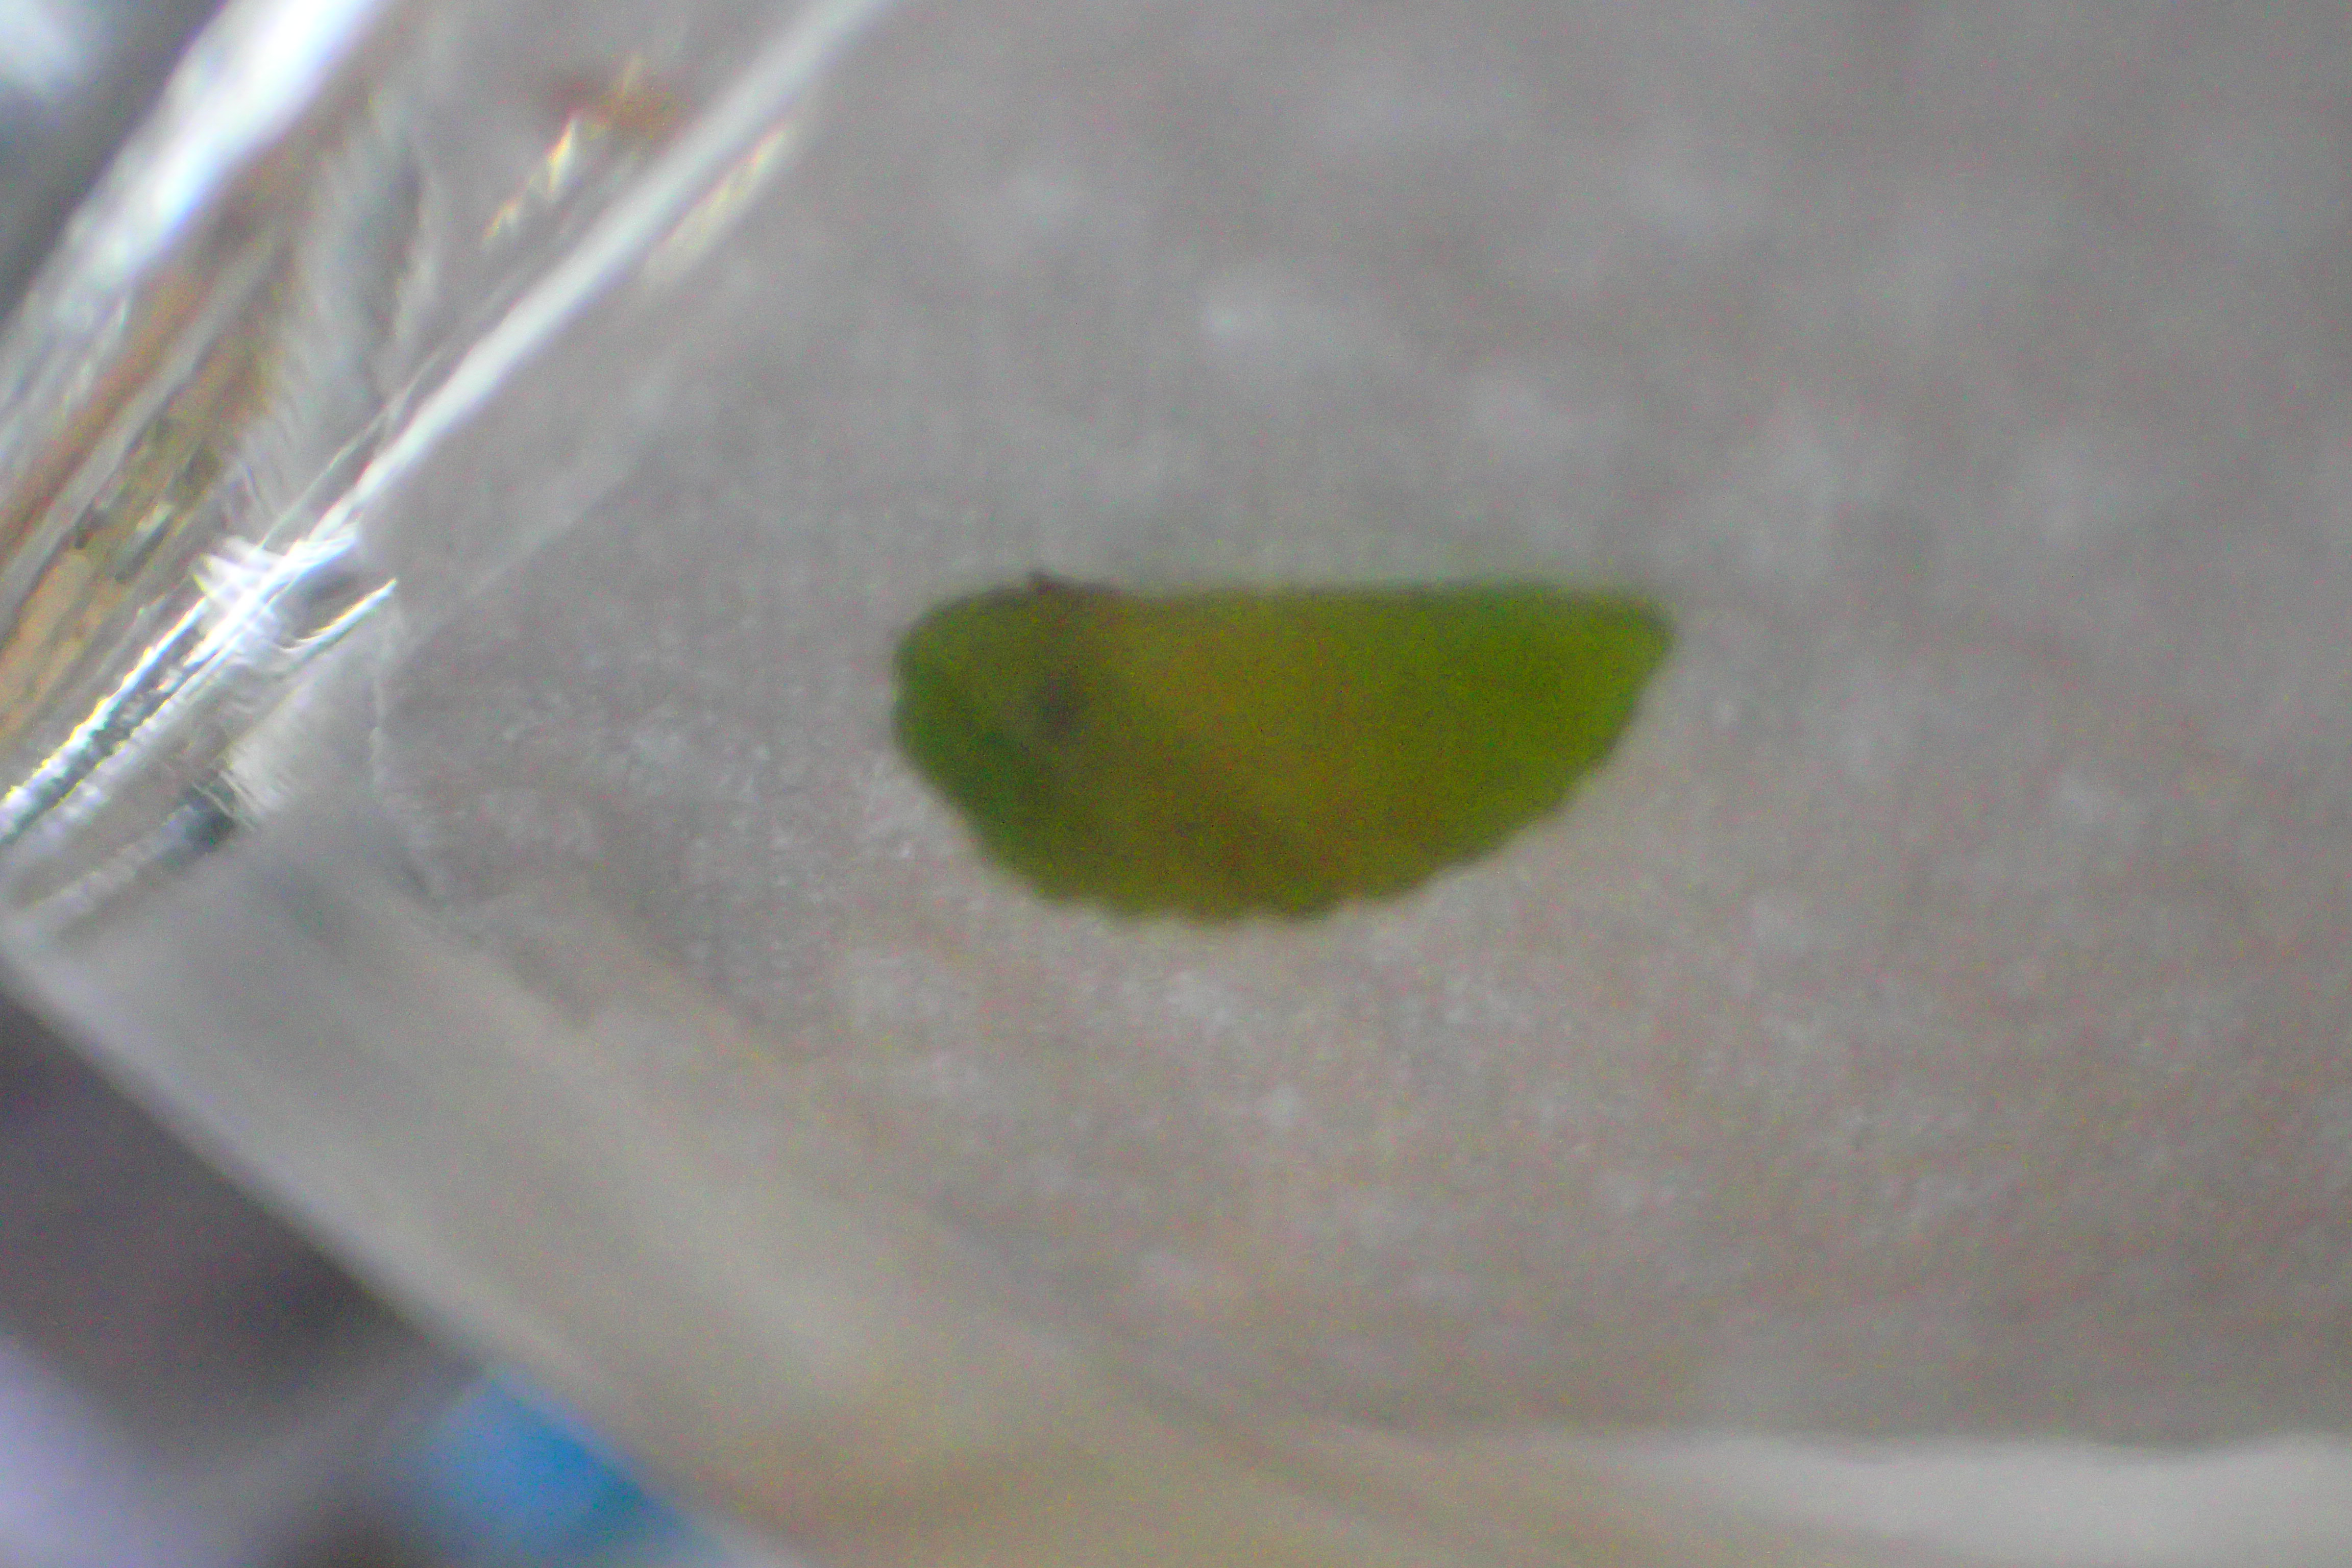
\includegraphics[width=5cm]{photo3/Larva4_prePupa.JPG}
  \end{center}
  \caption{前蛹が寄生されている可能性}
\end{figure}

\section{5/17の記録}
\subsection{12時:死亡判断}
もう完全に最初の2匹は動かないし, 明らかに干からびている. 死亡と判断した.
\begin{figure}[htbp]
  \begin{minipage}{0.5\hsize}
    \begin{center}
      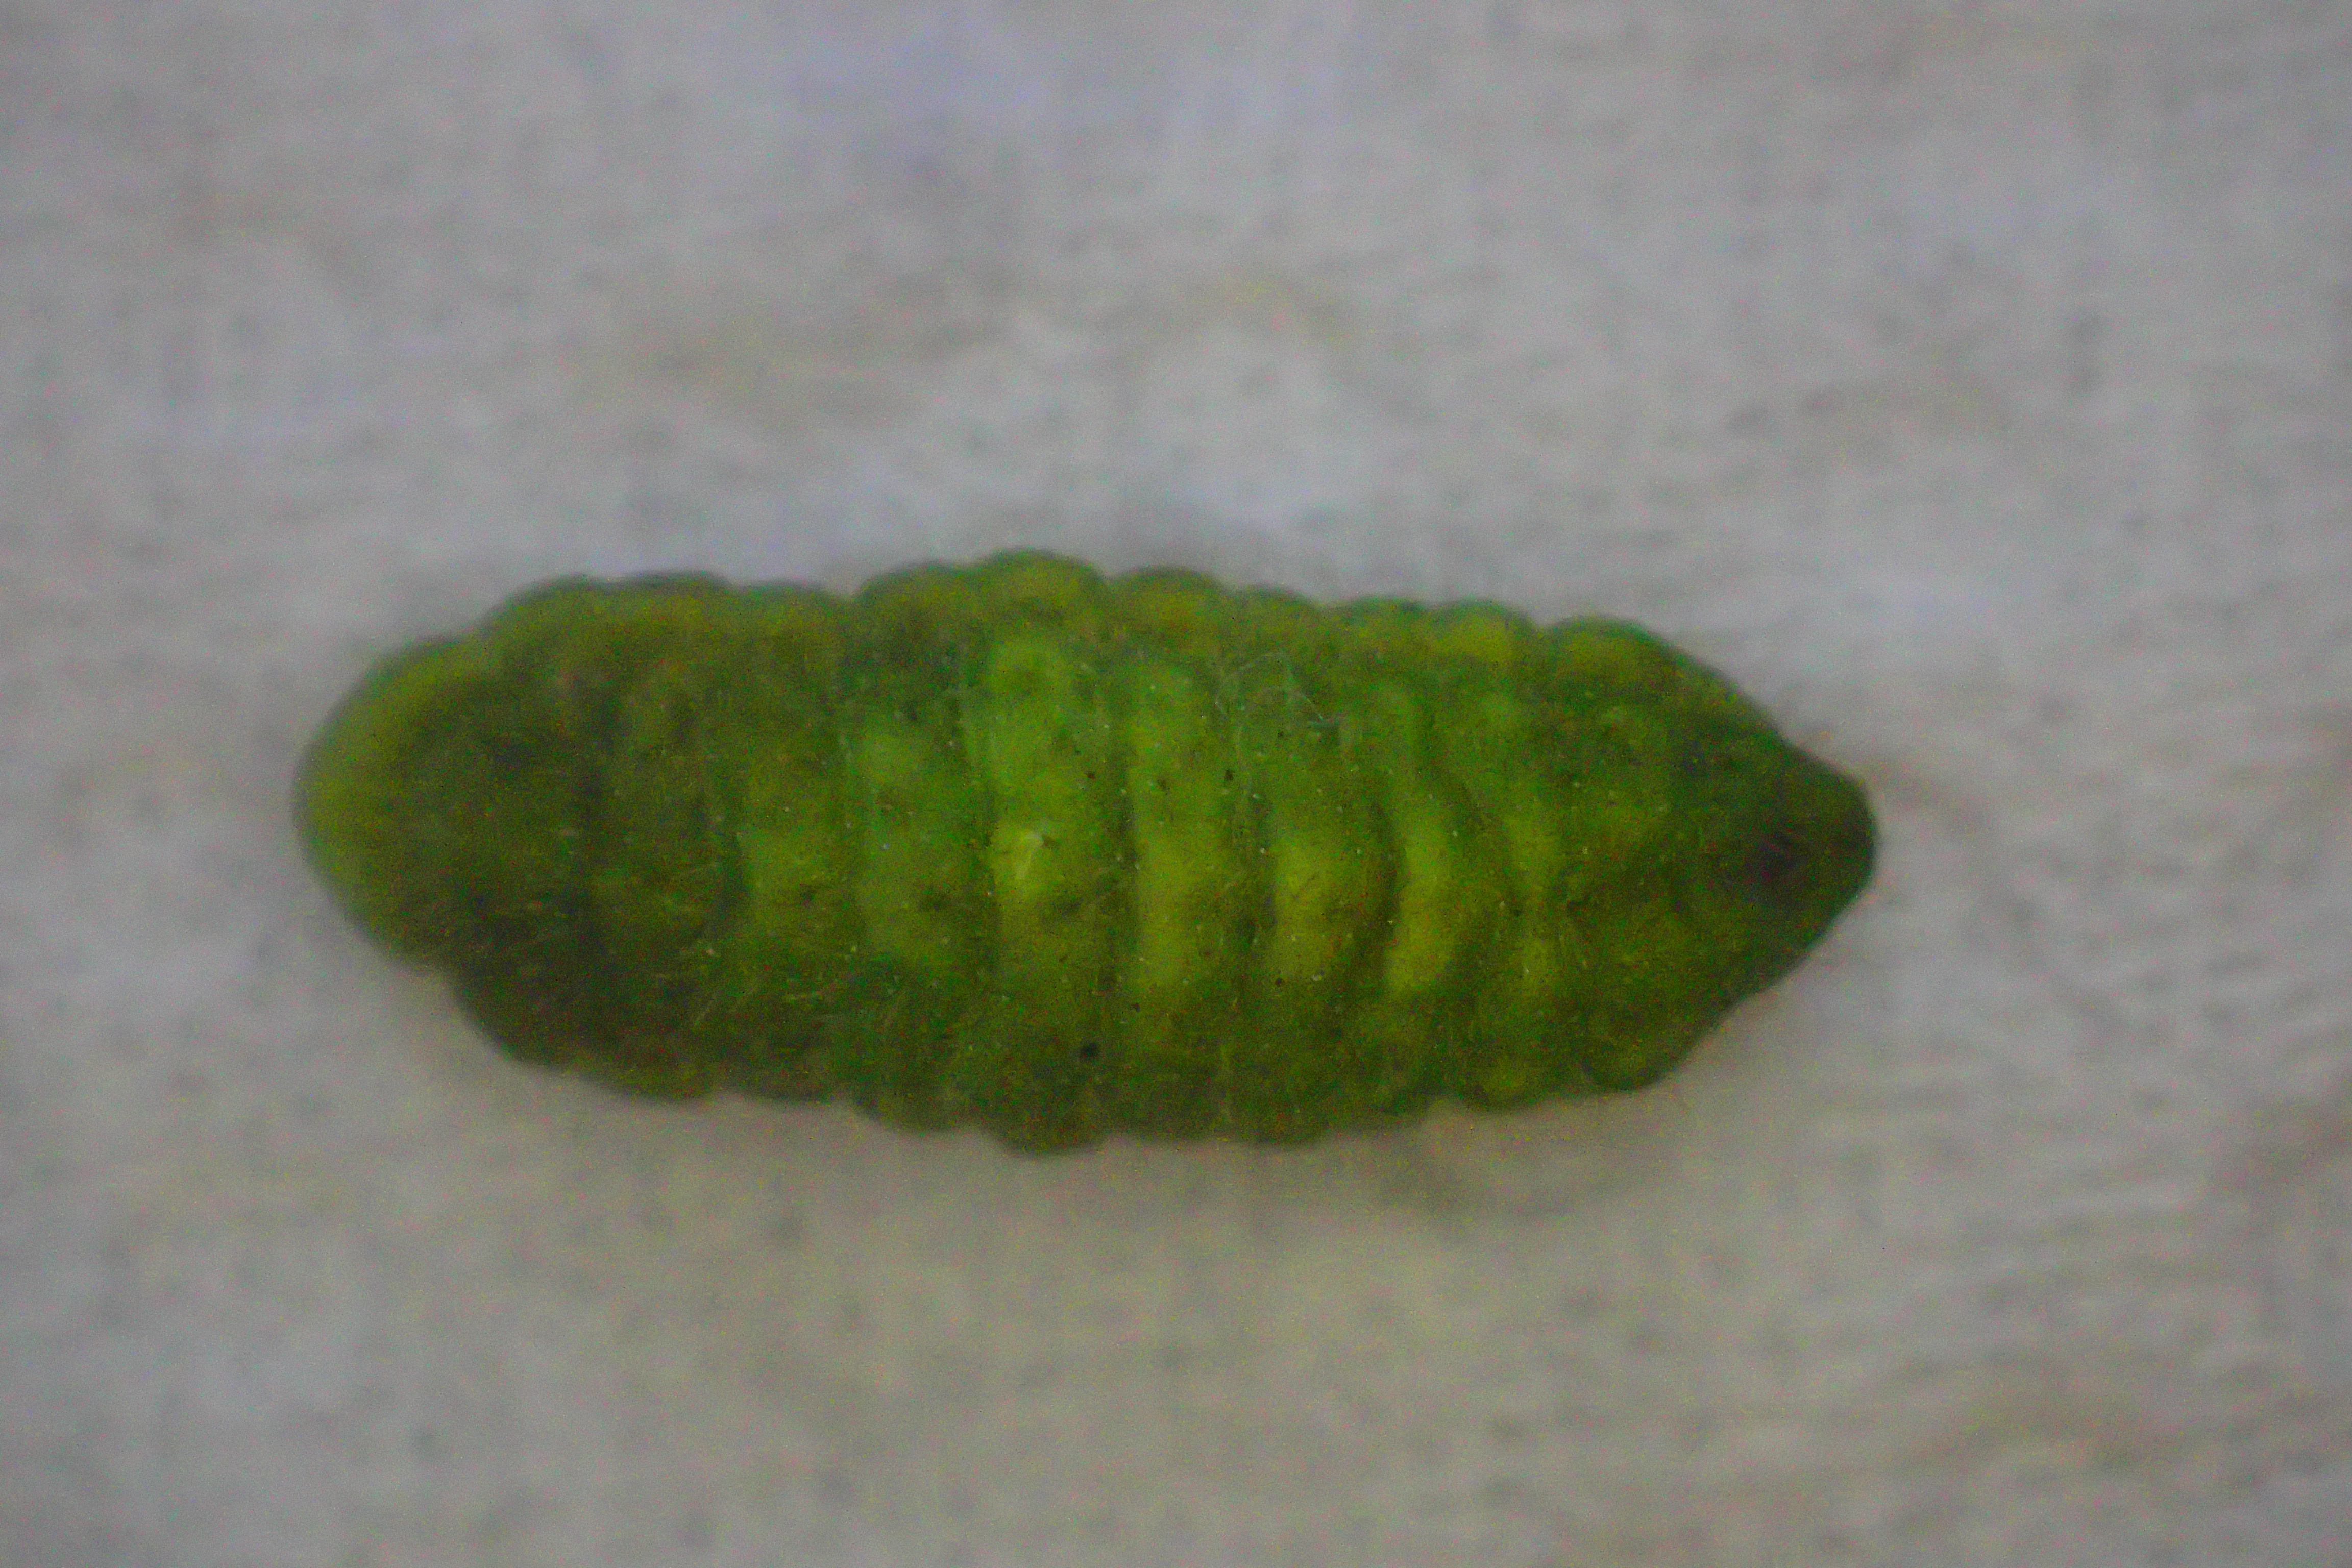
\includegraphics[width=5cm]{photo4/Larva1Dead.JPG}
    \end{center}
    \caption{幼虫1の死亡}
    \label{Larba1Dead}
  \end{minipage}
  \begin{minipage}{0.5\hsize}
    \begin{center}
      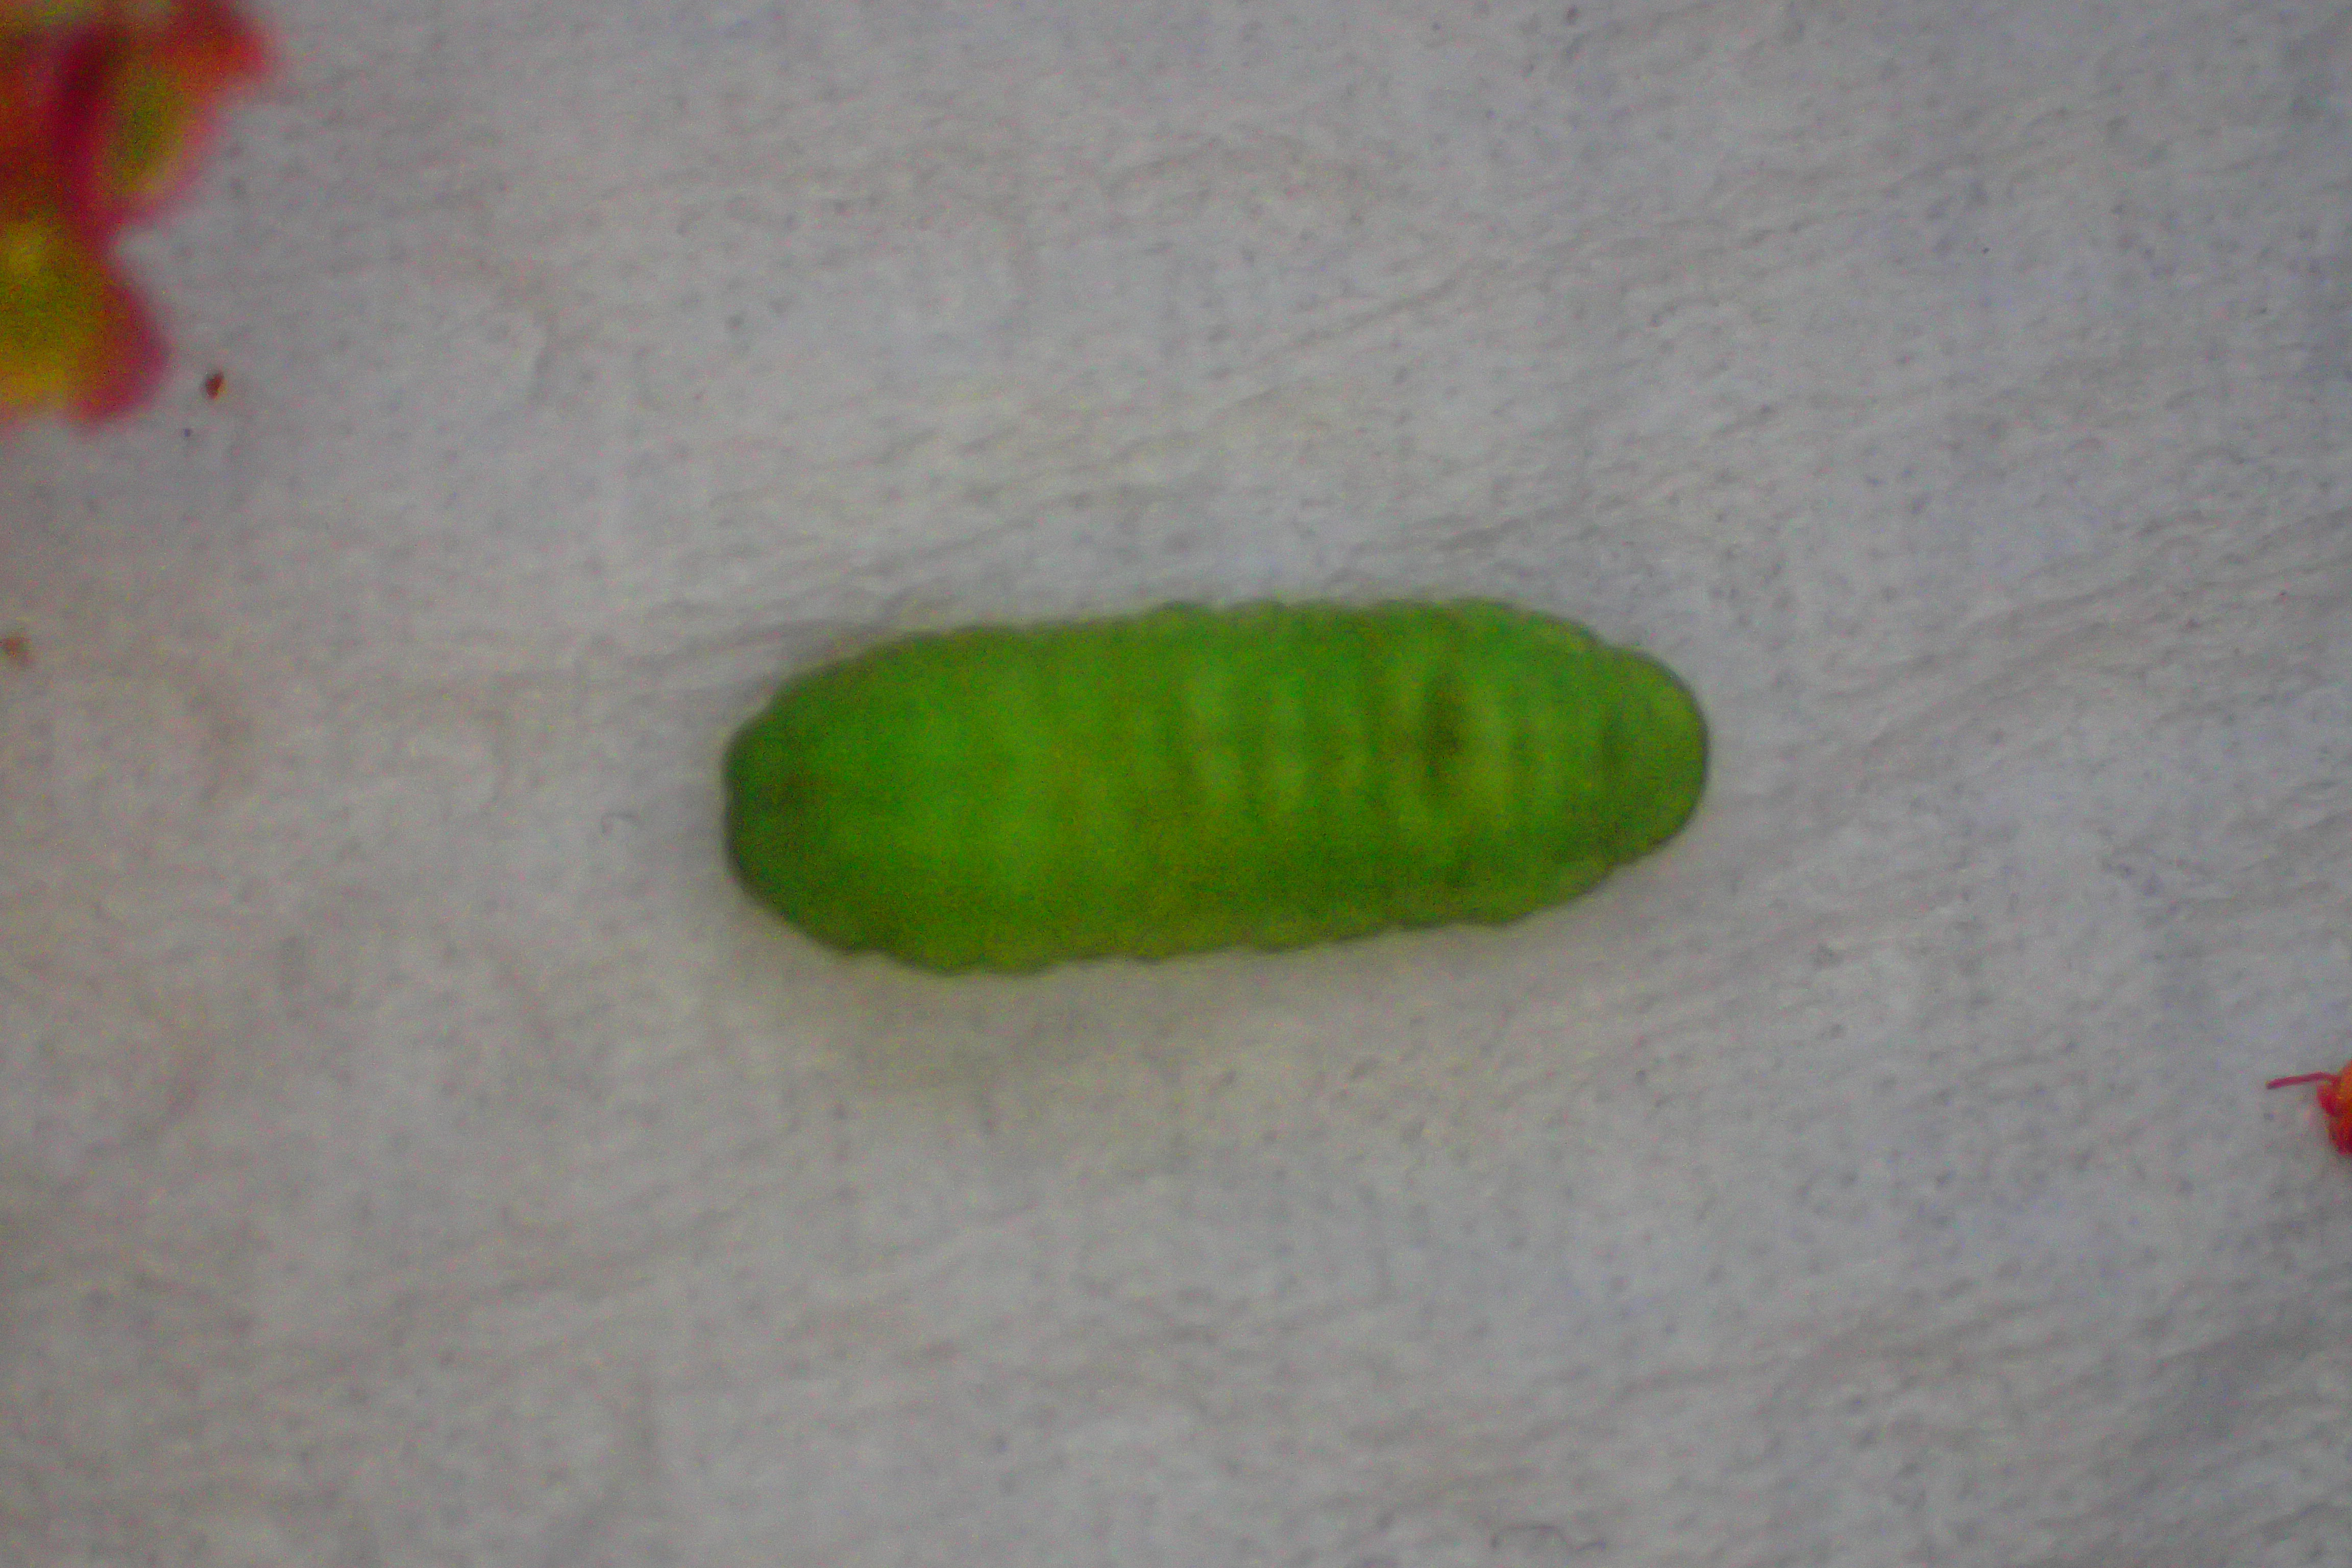
\includegraphics[width=5cm]{photo4/Larva2Dead.JPG}
    \end{center}
    \caption{幼虫2の死亡}
    \label{Larba2Dead}
  \end{minipage}
\end{figure}
前蛹になったやつは, ますます色が黄色がかってきており, 黒い斑点も大きくなってきた. 
おそらく, 中にハチ, もしくはハエがいる. 
\begin{figure}[htbp]
  \begin{center}
    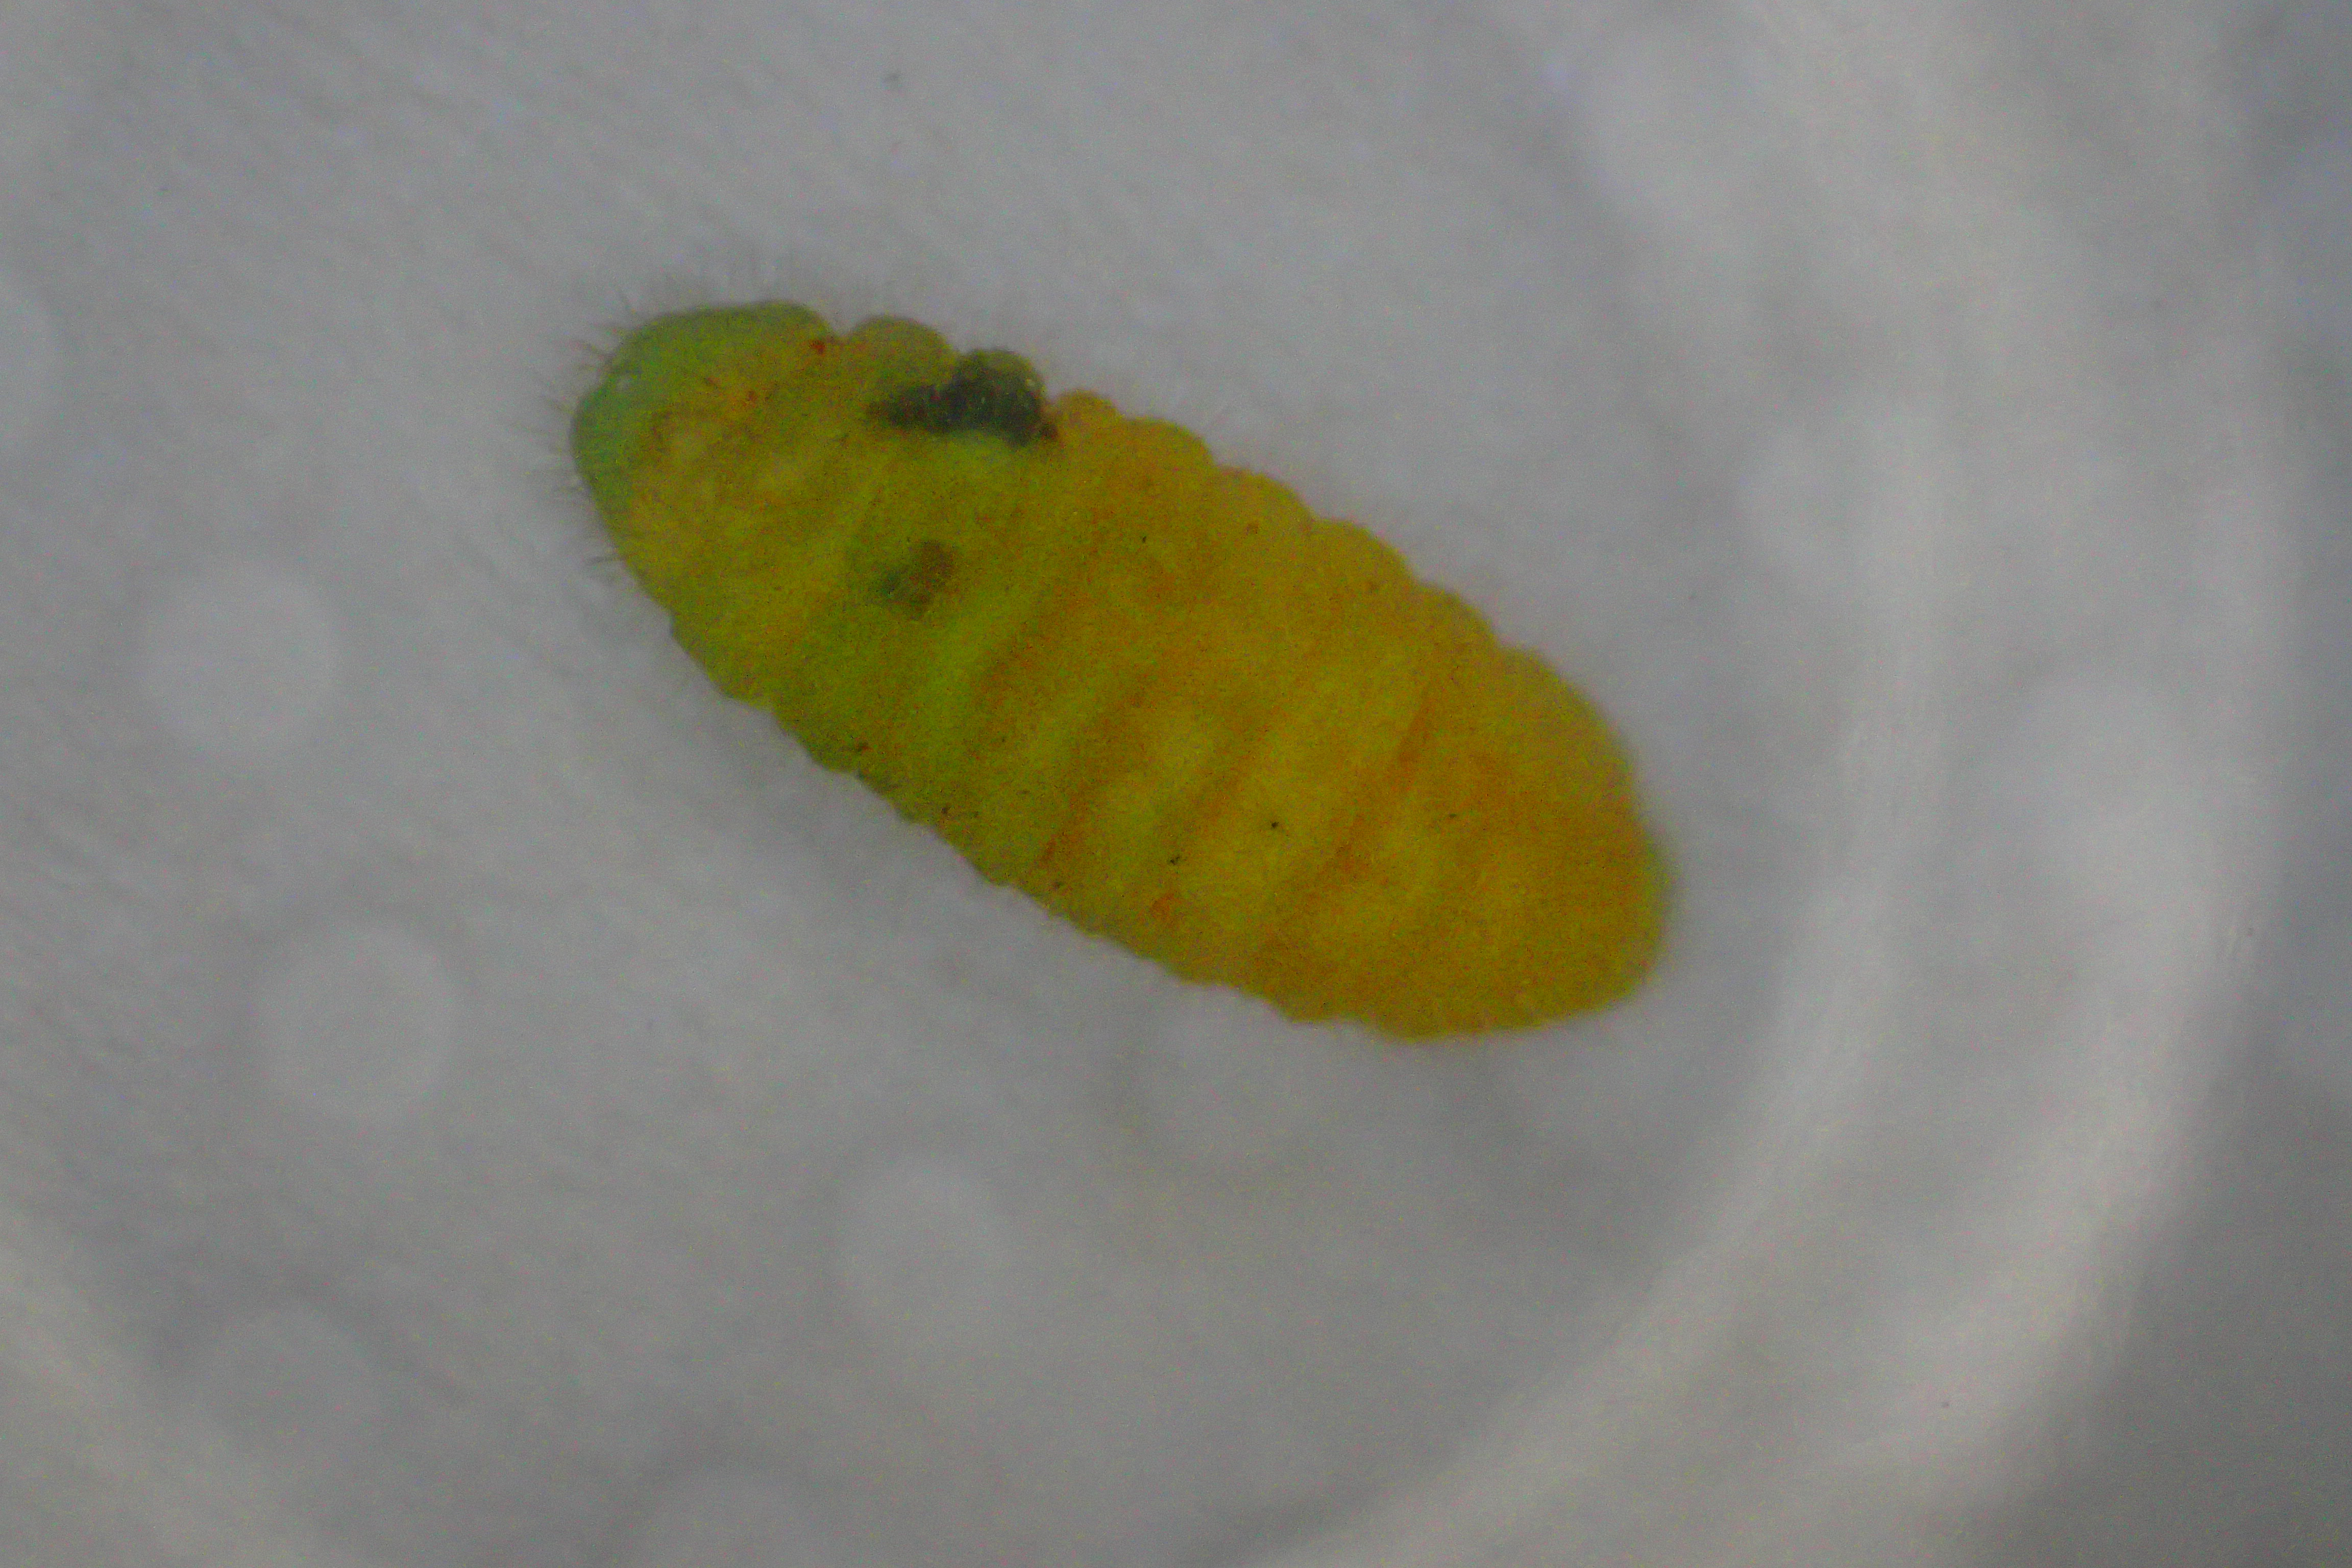
\includegraphics[width=5cm]{photo4/pupa_parasited.JPG}
  \end{center}
  \caption{前蛹が黄色く変色し, 黒い斑点が目立つようになってきた}
\end{figure}

\subsection{15時:2匹確保}
四季の森公園にて, 計3匹の幼虫を見つけた. 一匹はおそらく終齢, もう2匹は2齢程度. 2齢のうち1匹は, 捕獲中に落下してしまったので, 計2匹捕獲. 終齢は, 例のごとく花に貪りついていたが, 2齢の幼虫はどちらも割と苗の中段付近の枝で見つかった. 
割と, 若い幼虫のほうが, 葉裏にいるのかもしれない. 
\begin{figure}[htbp]
  \begin{minipage}{0.5\hsize}
    \begin{center}
      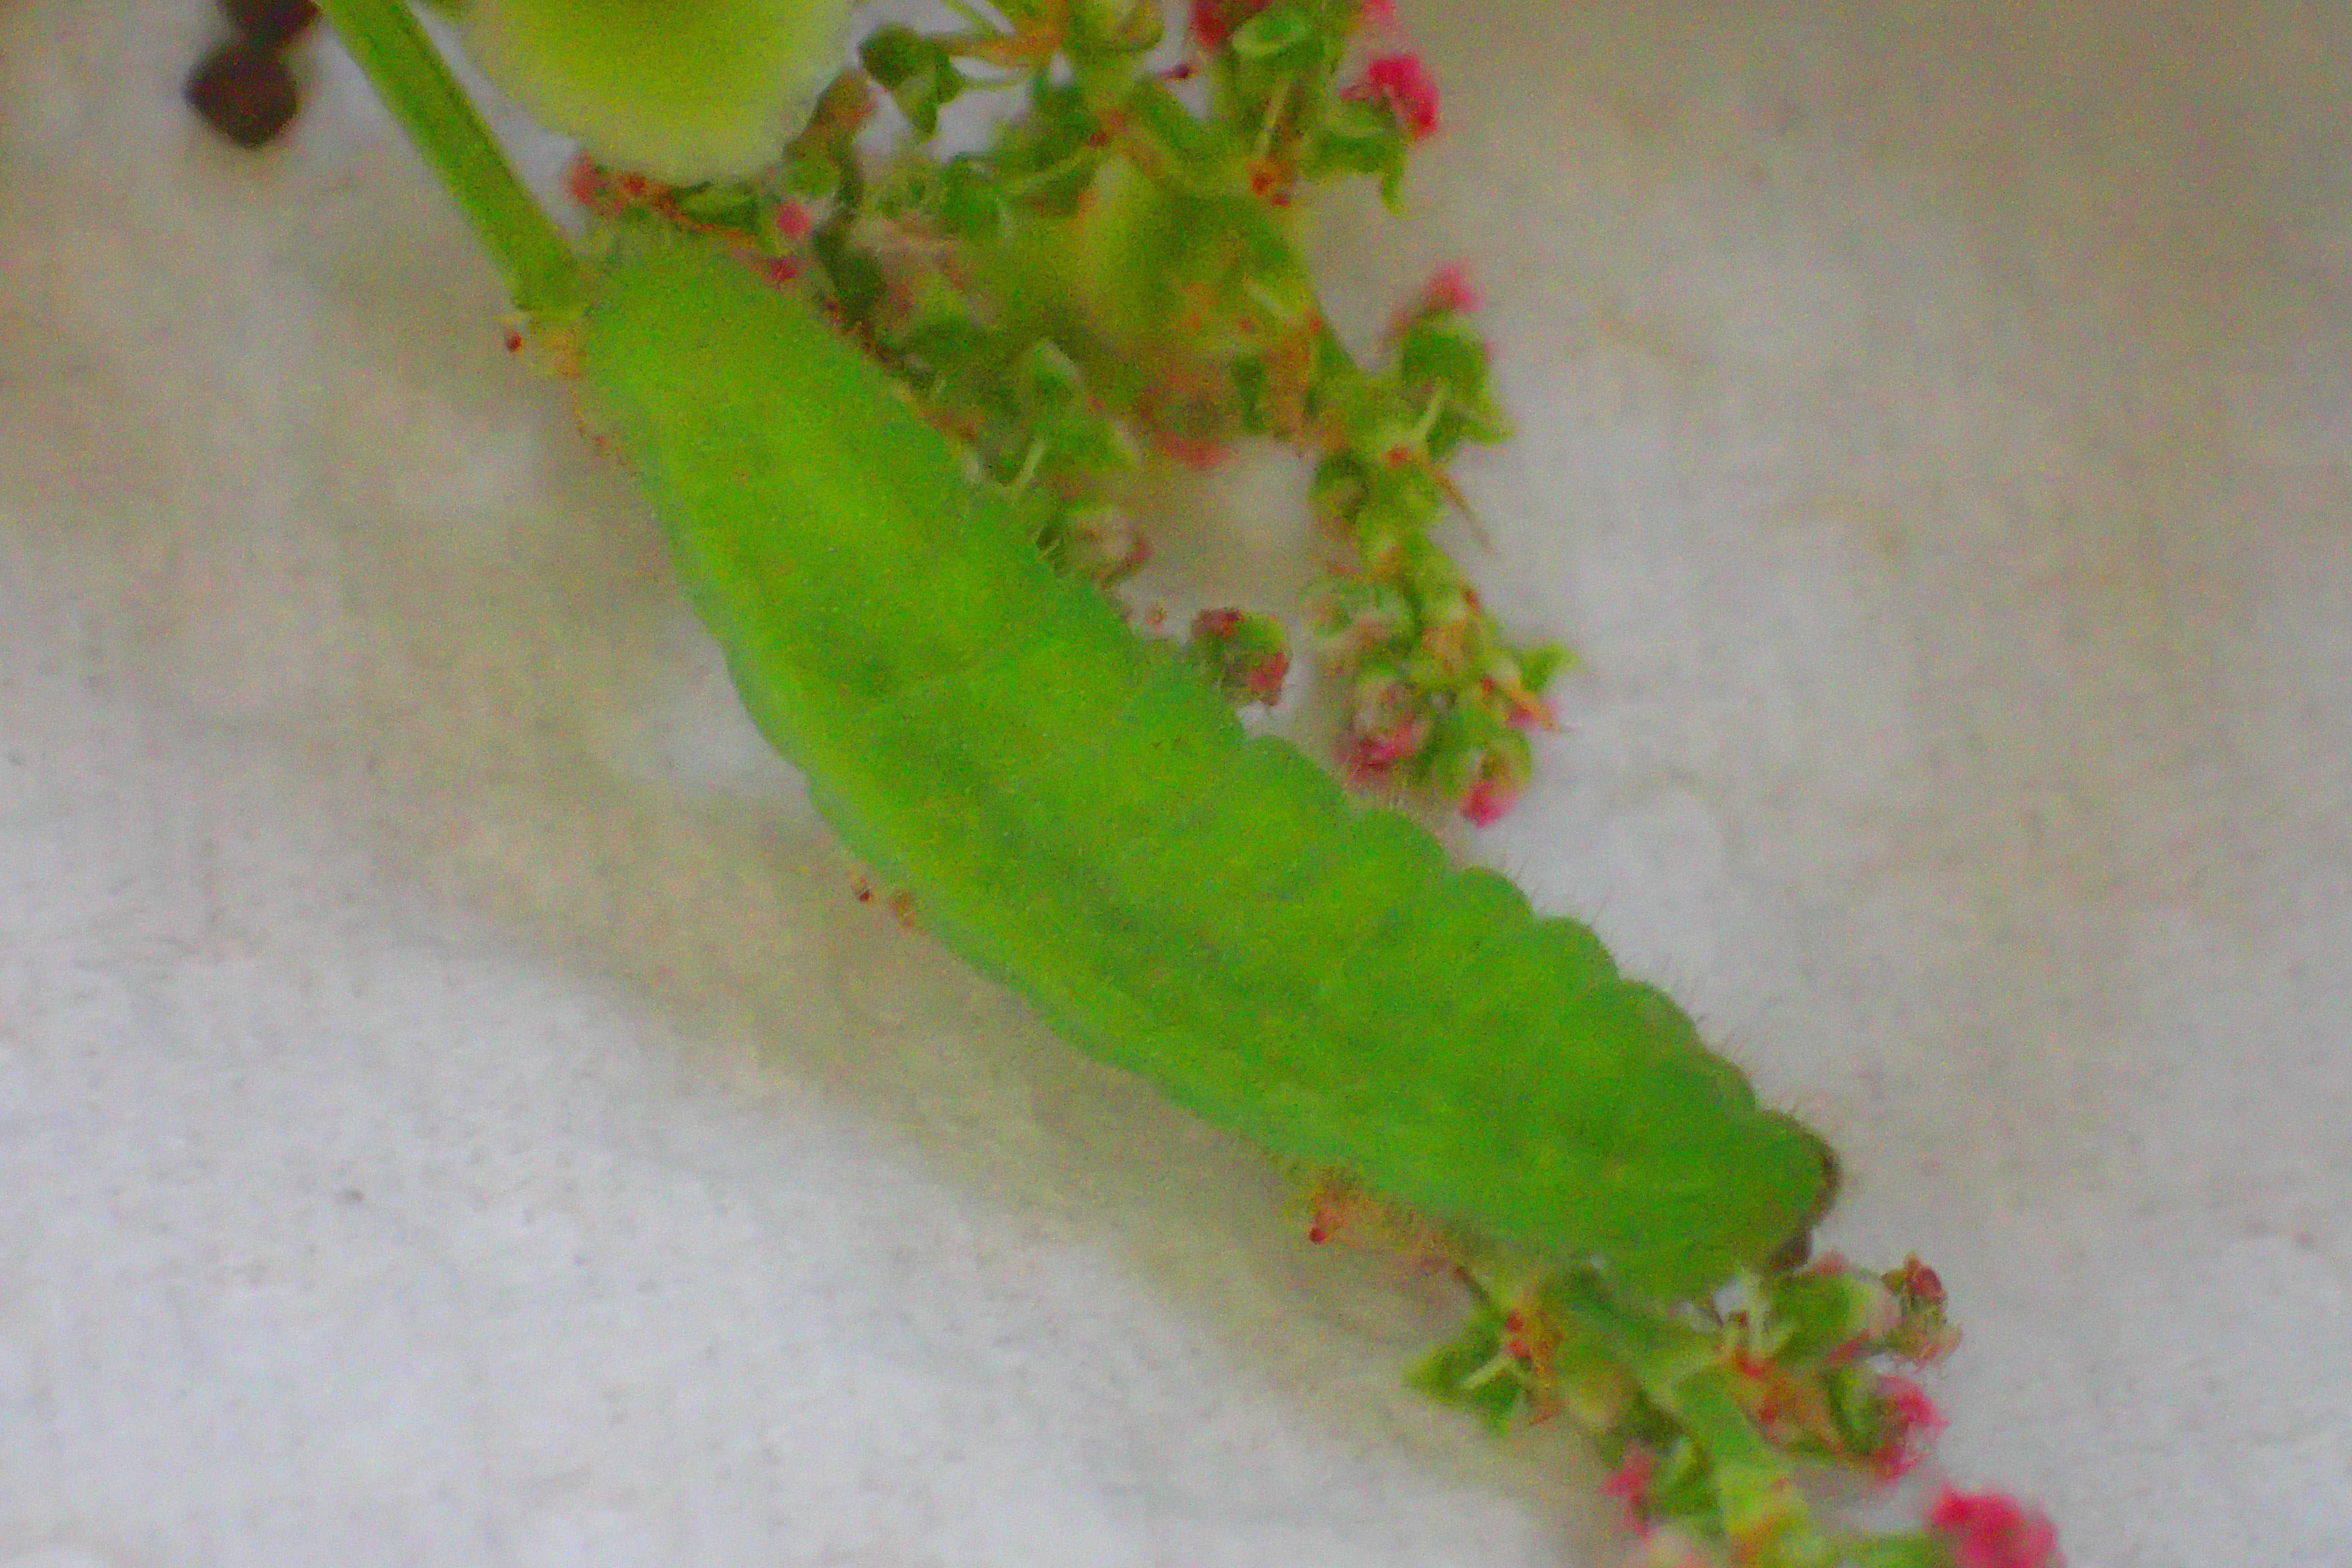
\includegraphics[width=5cm]{photo4/Larva5.JPG}
    \end{center}
    \caption{幼虫5}
  \end{minipage}
  \begin{minipage}{0.5\hsize}
    \begin{center}
      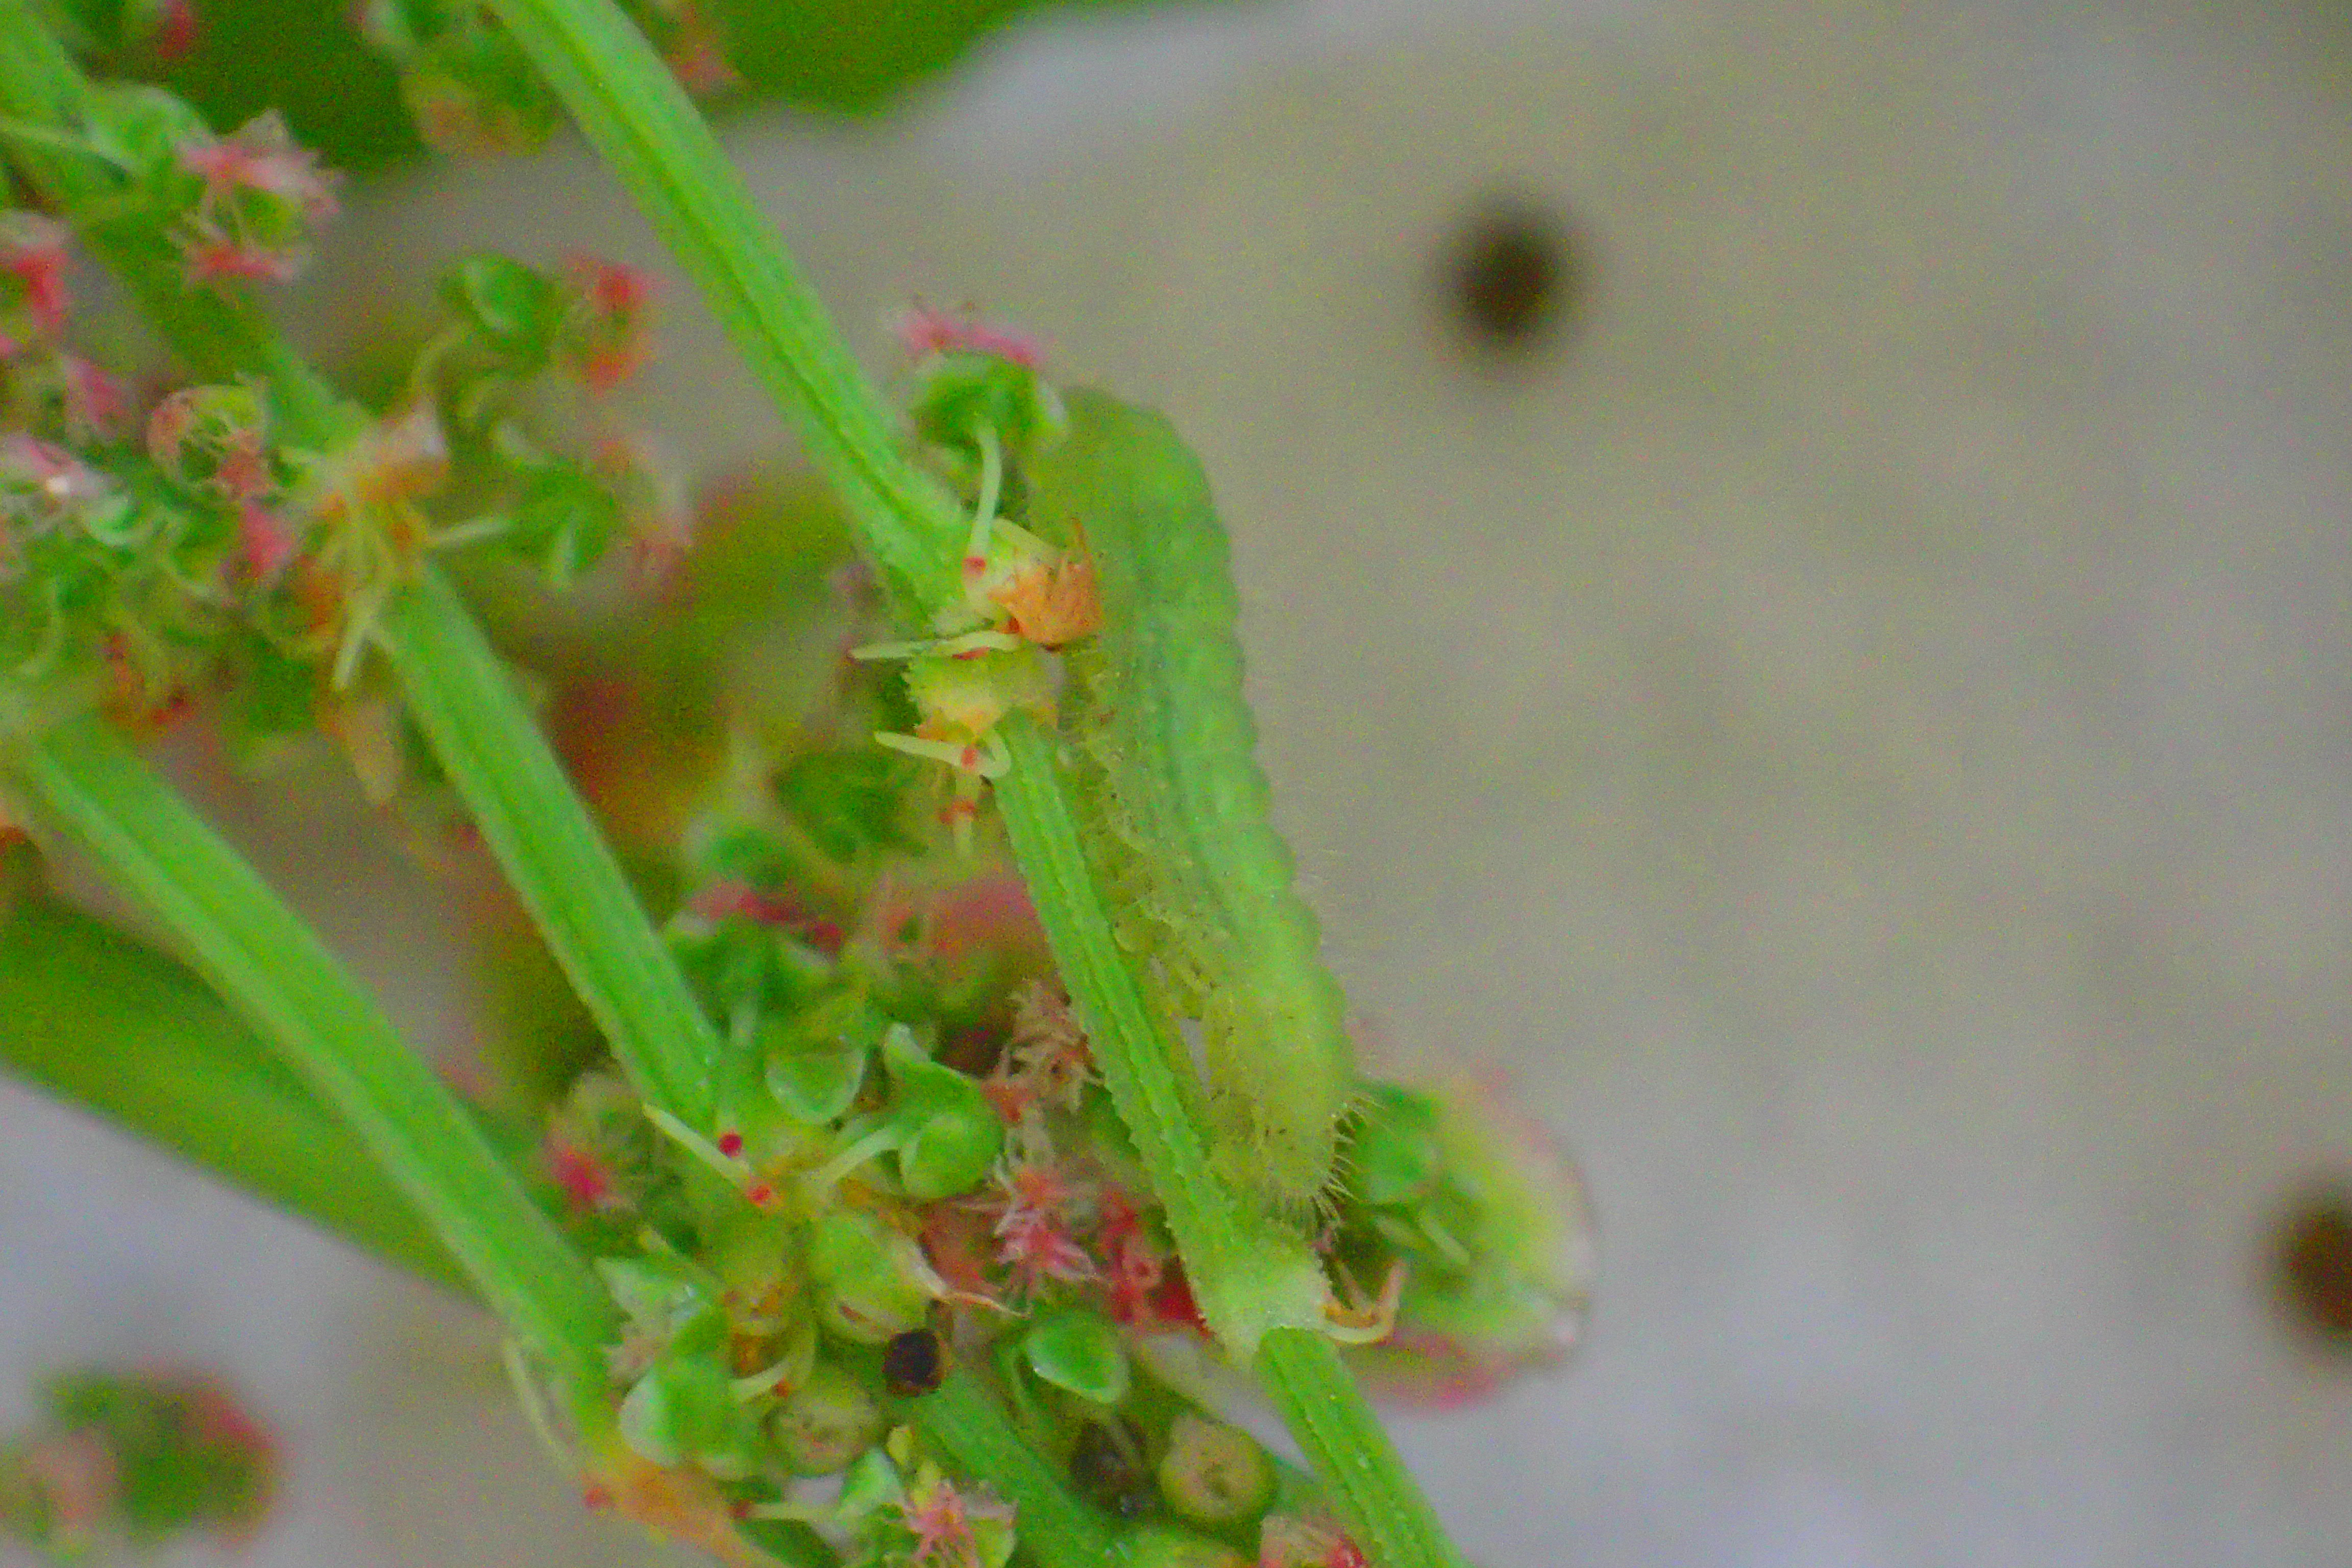
\includegraphics[width=5cm]{photo4/Larva6.JPG}
    \end{center}
    \caption{幼虫6}
  \end{minipage}
\end{figure}

\subsection{16時:蛆虫がでてきた}
前蛹を別ケースに移動しておいたが, ケースを見ると, 黄色い蛆虫が高速に移動していた. 
もう少し気づくのが遅かったら, 家の中を這っていたことだろう. 
案の定, 黒い斑点があったところに穴が空き, 蛆虫が出てきたようだ. 
ハエかハチか, 正体を見極めてもいいが, そこまでするのもケースの無駄なので, 水中で死んでもらうことにした. 
\begin{figure}[htbp]
  \begin{minipage}{0.5\hsize}
    \begin{center}
      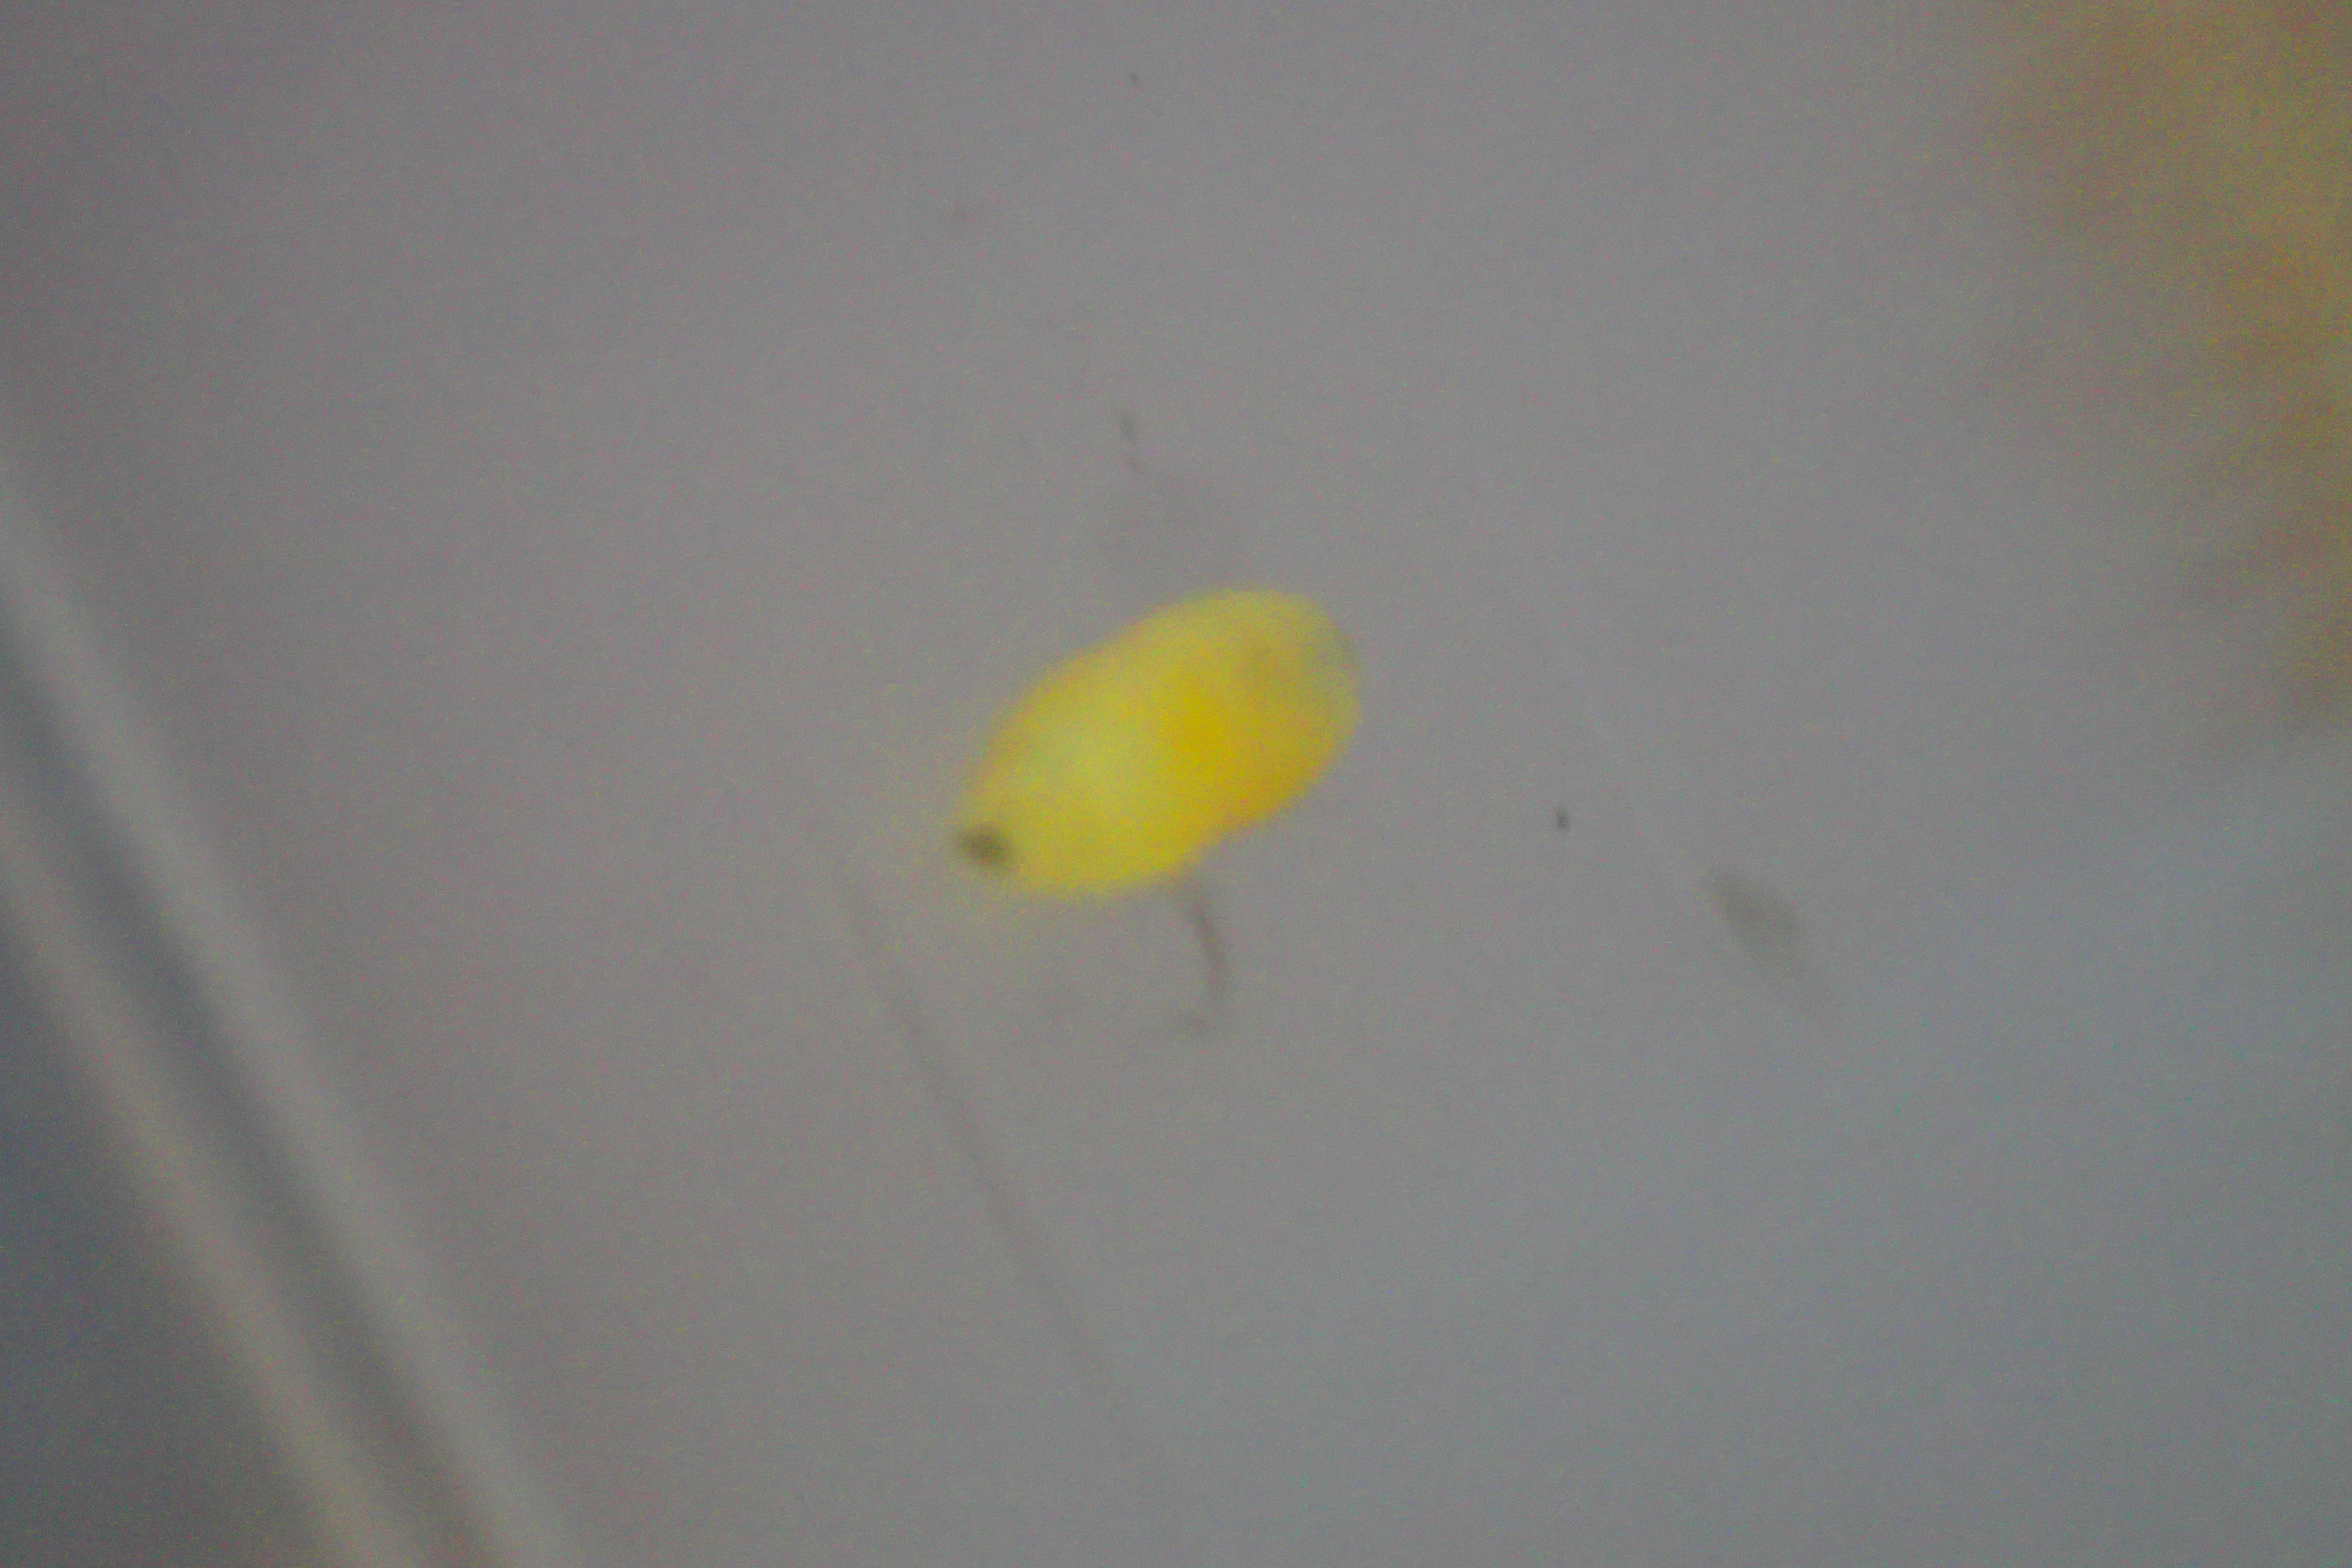
\includegraphics[width=5cm]{photo4/maggot.JPG}
    \end{center}
    \caption{蛆虫}
  \end{minipage}
  \begin{minipage}{0.5\hsize}
    \begin{center}
      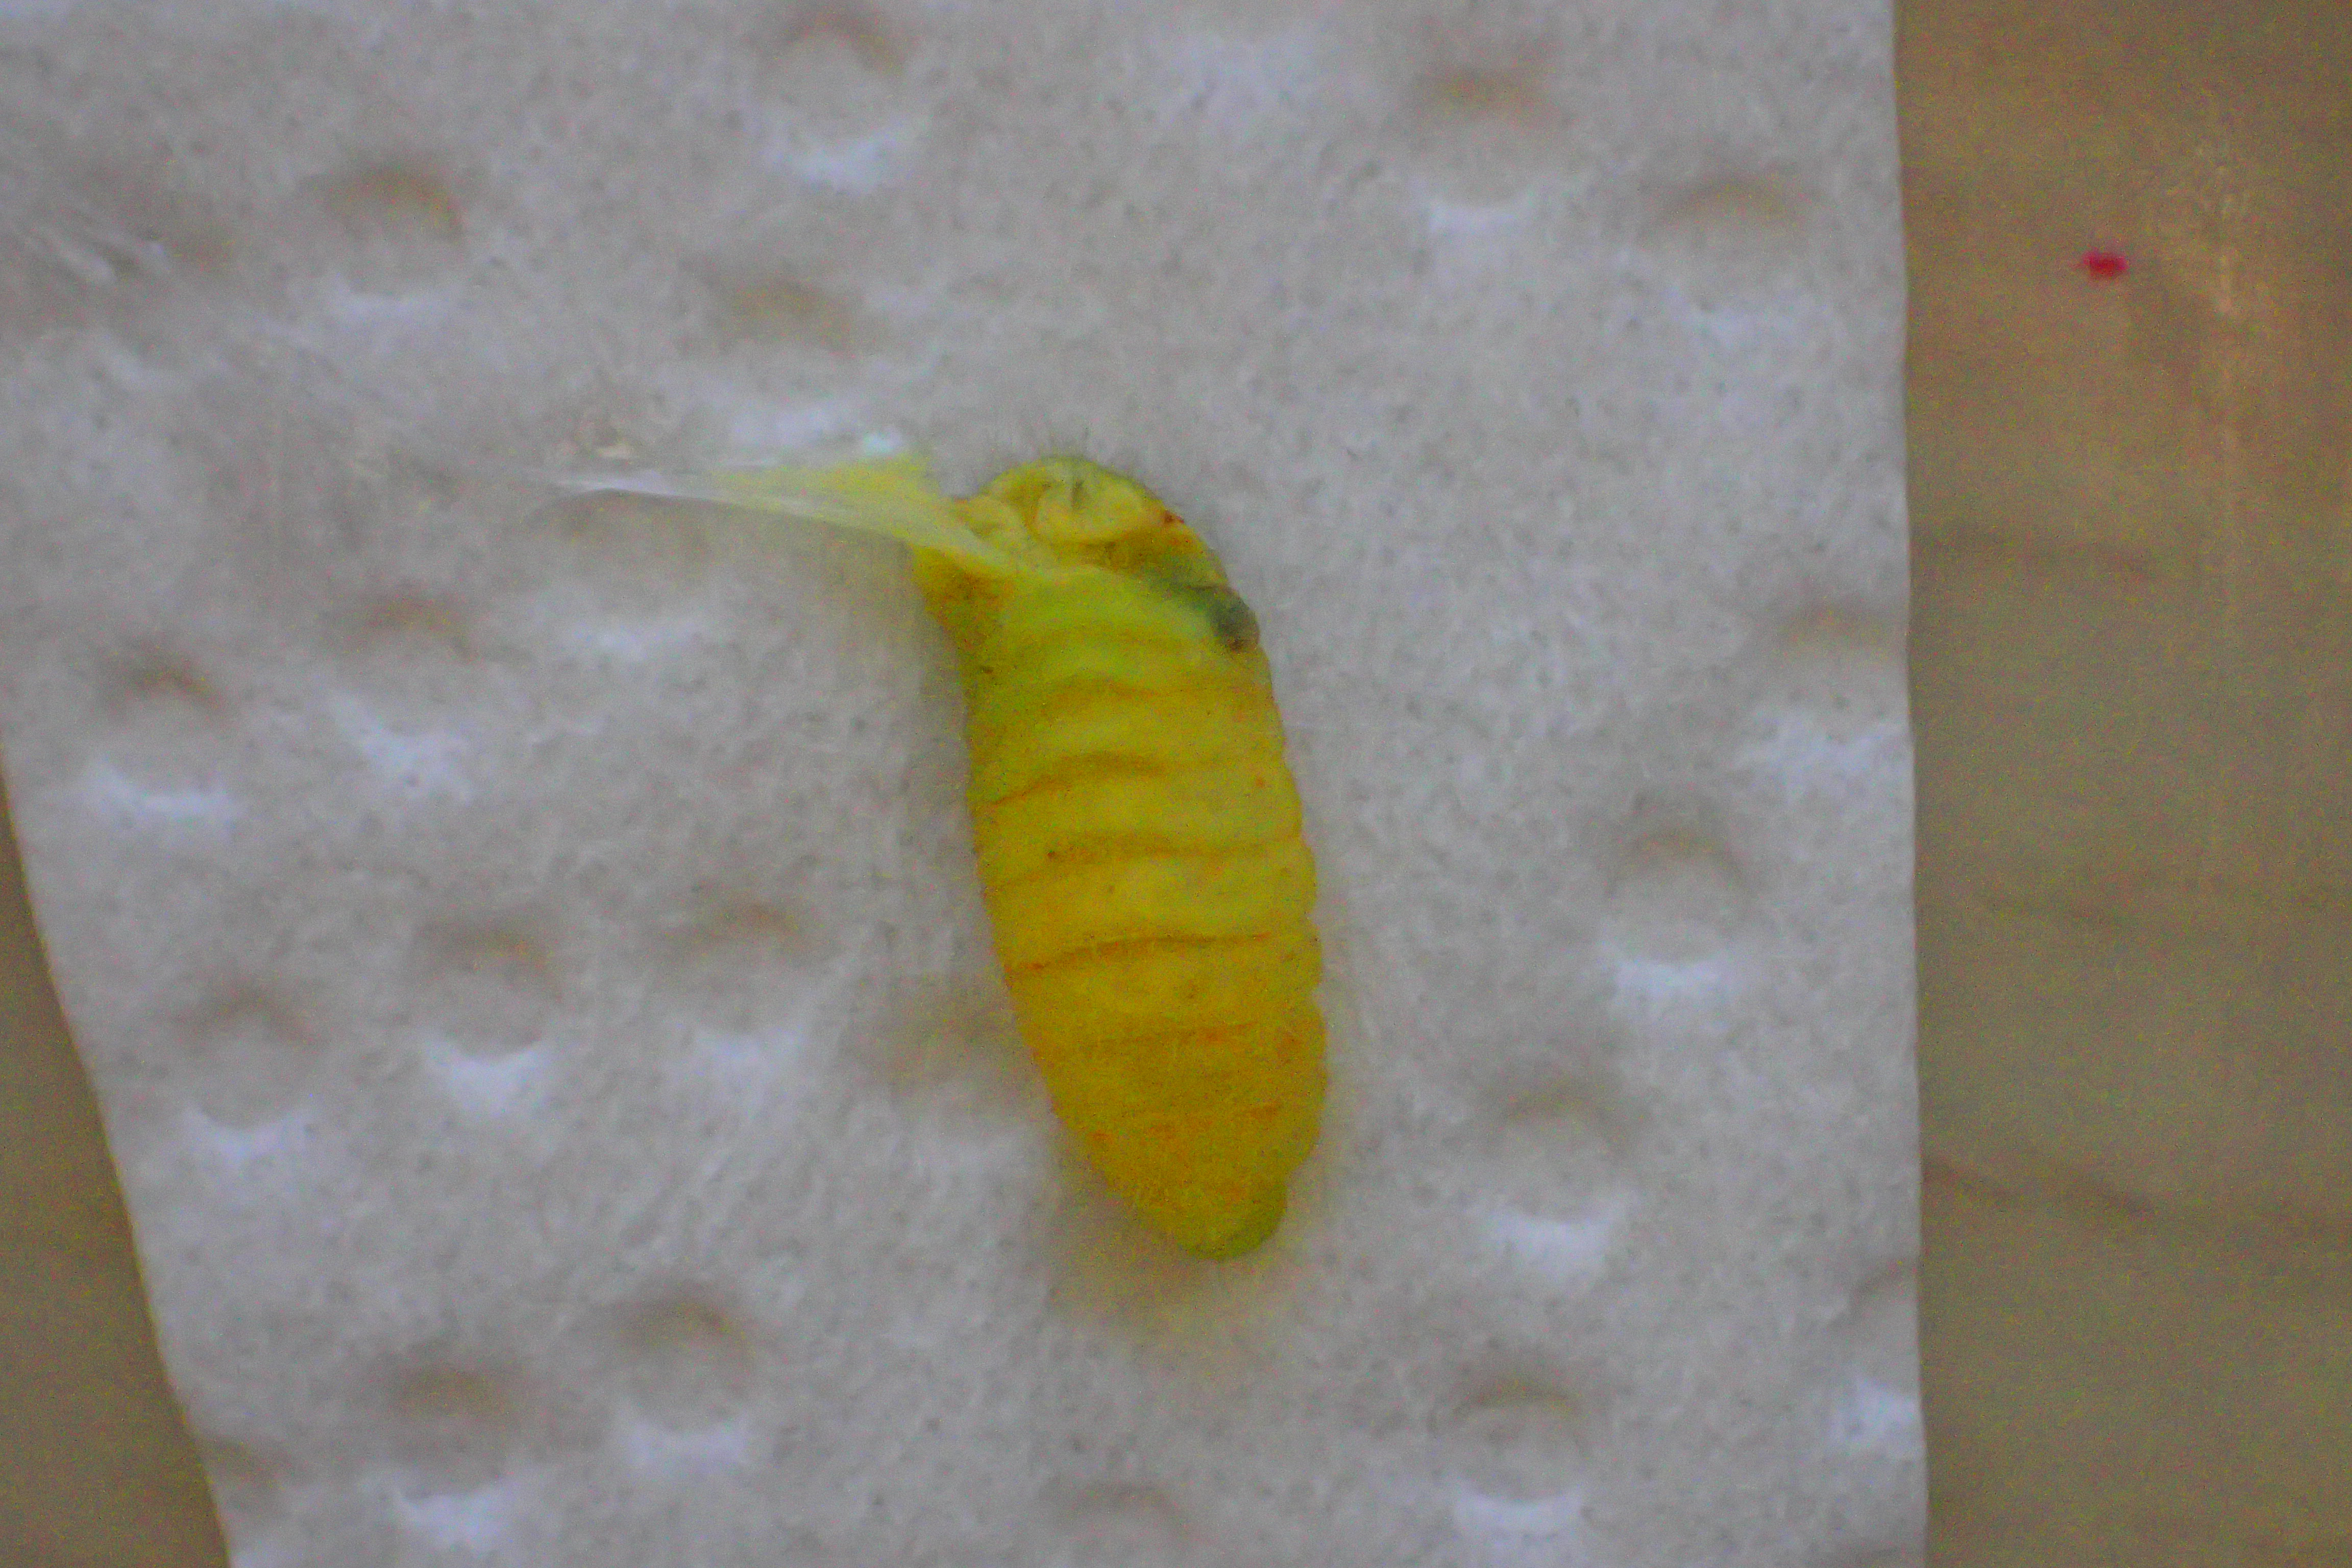
\includegraphics[width=5cm]{photo4/pupaDead.JPG}
    \end{center}
    \caption{寄生虫が出た後の蛹}
  \end{minipage}
\end{figure}

\subsection{17時:蛆虫がまだ生きている}
蛆虫の生命力の高さはしっていたが, 無酸素状態で1時間以上たっているのに, まだ水中で動いている. 
たいしたものだ. 

\subsection{22時:もう一匹が前蛹になった}
夕方より, 終齢の一匹が, やたらと食草を離れ, ケースの中をうろつくようになったので, 
もしかしたらと思っていたが, ガラスボウルの蓋に糸を貼り, 前蛹になった. 
今回は, 特にきになる斑点もないのと, たまたまガラスボウルに付いてくれたので, 観察がしやすく, 
体内を何かが蠢く様子もないので, おそらく成功だ. 
キッチンペーパーには, あちこちに, 水分を多量に含んだと思われる糞の痕跡があった. 
2時間程度全く動かなかったが, その後, 糸による足場の強化をし, 完全に動かなくなった. 
\begin{figure}[htbp]
  \begin{center}
    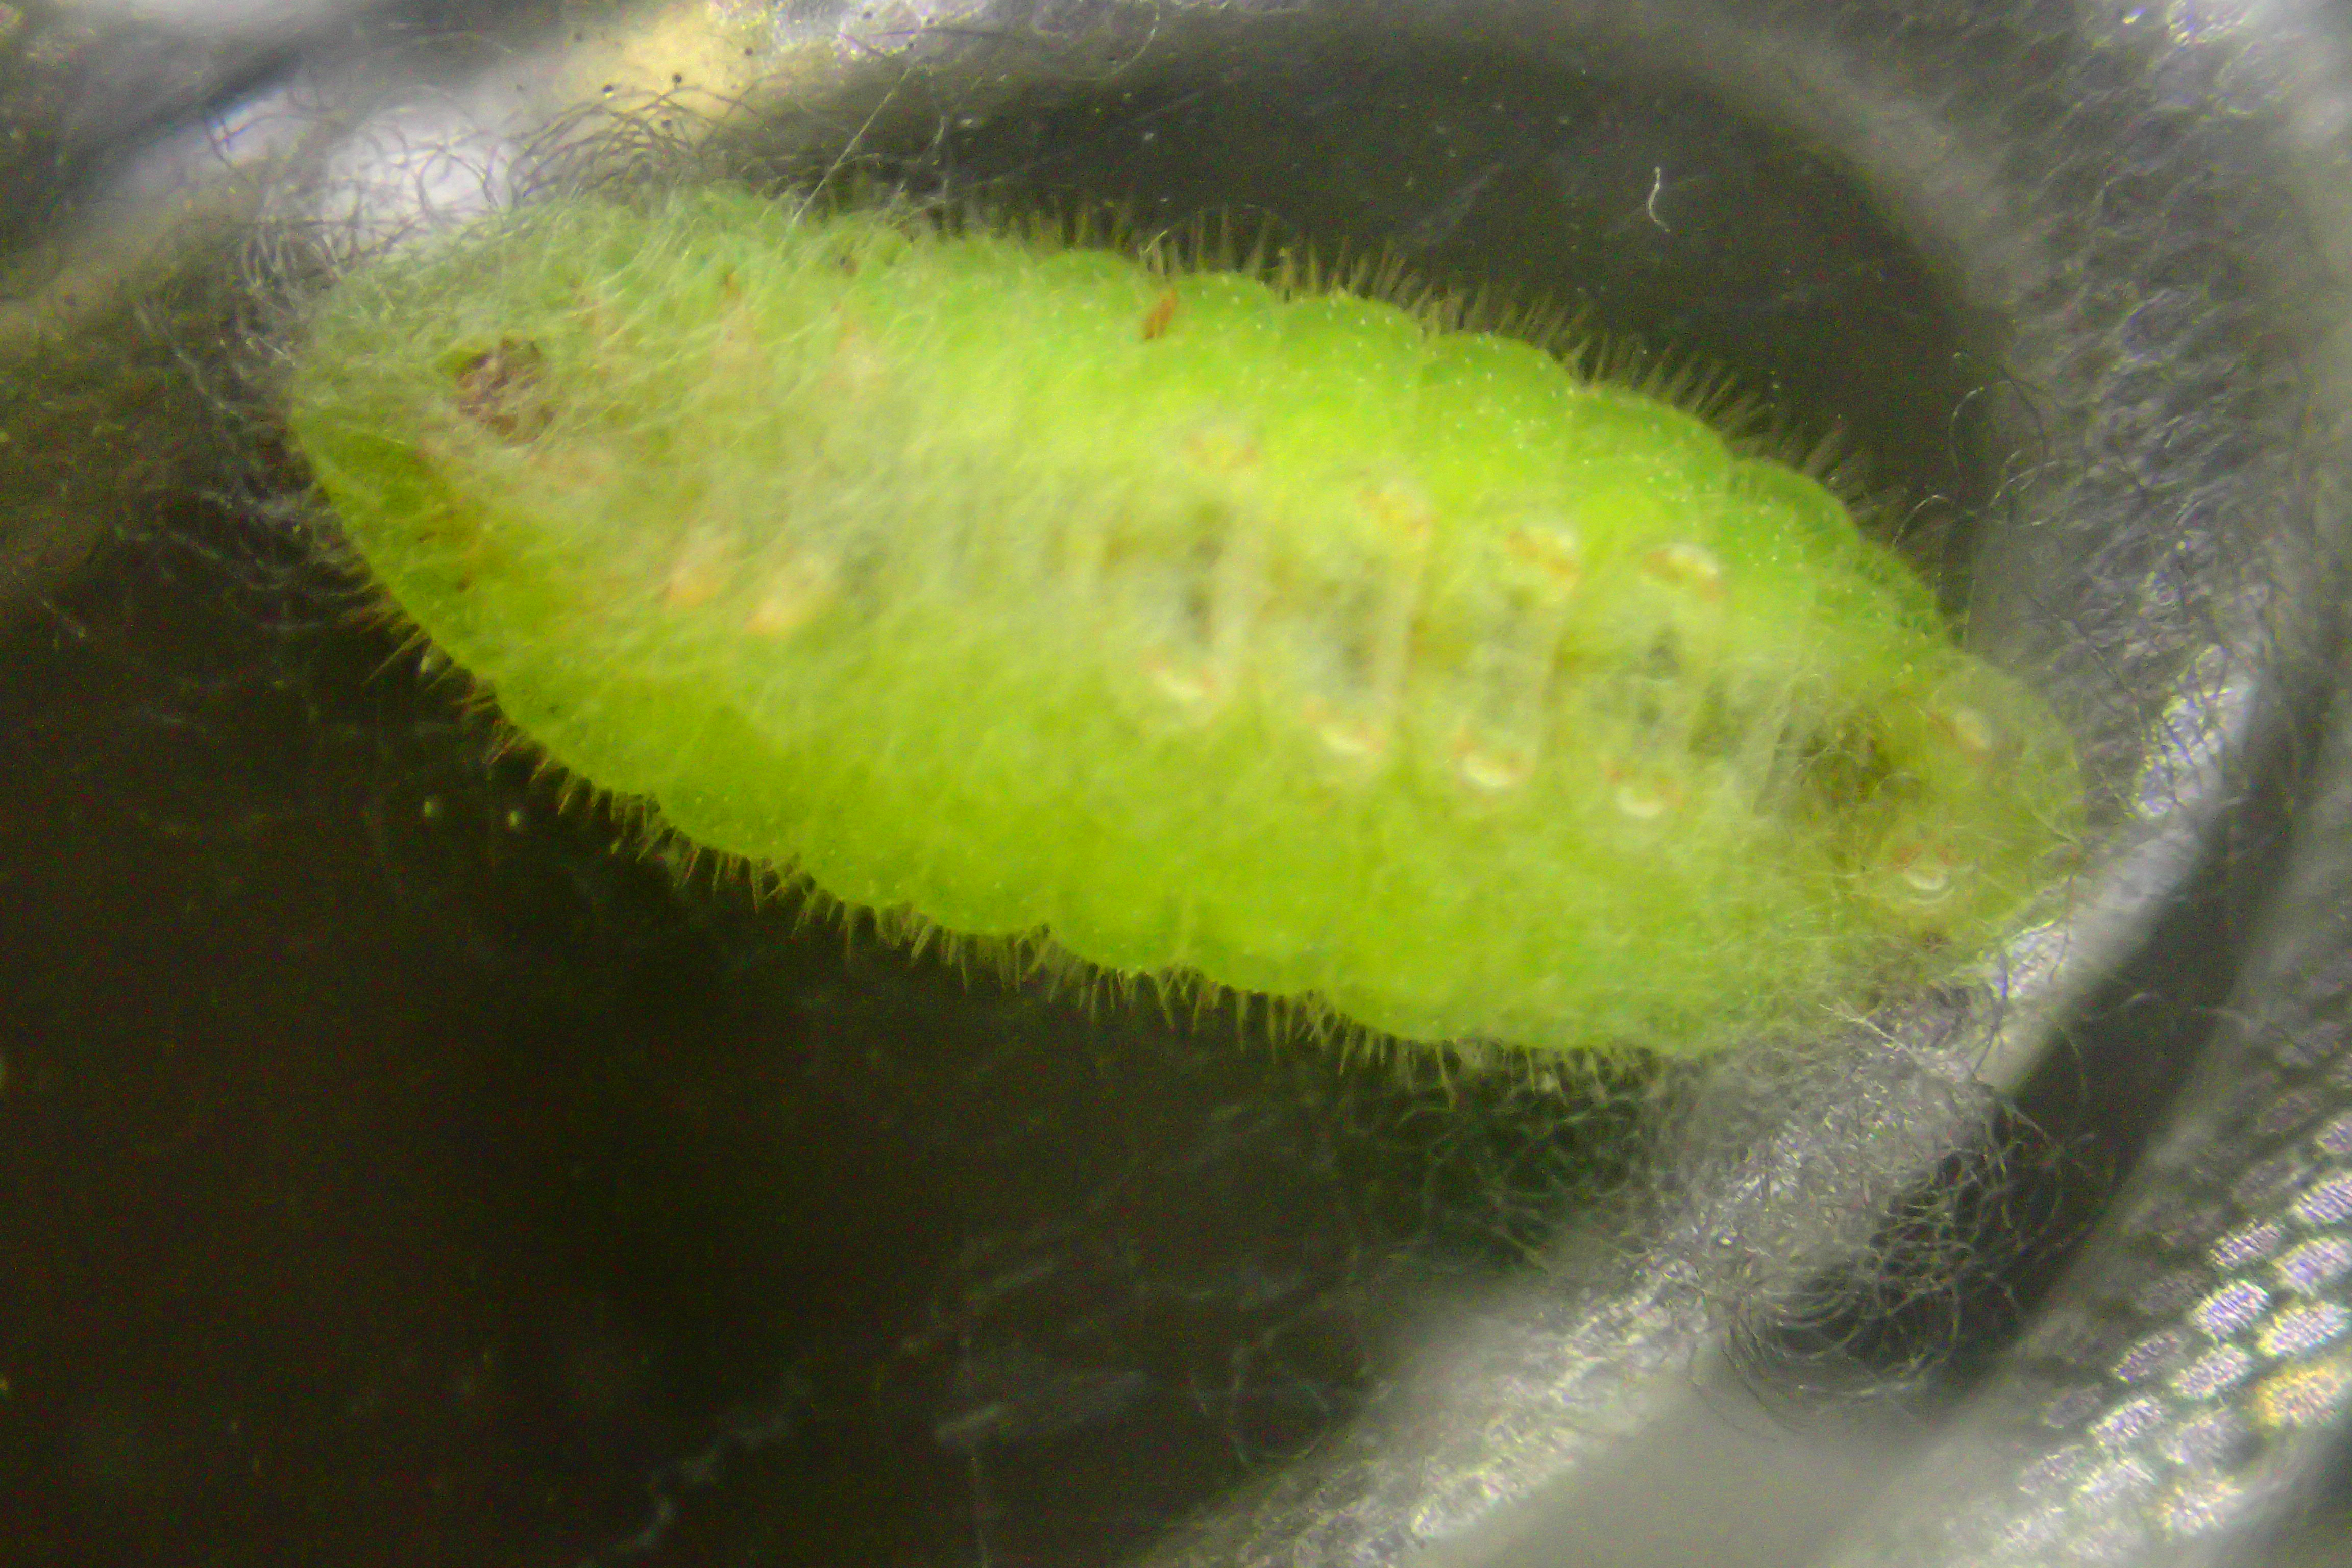
\includegraphics[width=5cm]{photo4/prePupa.JPG}
  \end{center}
  \caption{もう一匹が前蛹になった}
\end{figure}

\subsection{23時:さらにもう一匹が前蛹になった, と思われる}
もう一匹の終齢幼虫が, 少し気になる動きをした. 先に死んだ2匹にも見られた動作だが, 
丸まったり, 伸びたり, という, もがいているようにも見える動作である. 
これは, こいつも危ないか, と思っていたが, その後動作は落ち着いたようで, ただ, キッチンペーパーの上に落ち着いていた. 
よく見ると, 頭部付近に, 細い筋が見られ, おそらく, 体を固定する糸ではないかと思われる. 
光を当てても反応しないし, 尾の方を見ると, 水分を出した糞の跡があり, うまくいっていれば, 前蛹, 
ダメであれば, 寄生中が体内でうごめき出した可能性がある. 
いずれにしろ, 明日になればわかる. 
\end{document}
